\documentclass[a4paper,12pt]{article}

% --- Idioma y codificación ---
\usepackage[utf8]{inputenc}   % Acentos directos
\usepackage[T1]{fontenc}      % Codificación de salida
\usepackage[spanish]{babel}   % Español
\usepackage{lmodern}          % Fuente moderna

% --- Matemáticas ---
\usepackage{amsmath}          % Entornos matemáticos
\usepackage{amssymb}          % Símbolos
\usepackage{amsthm}           % Teoremas
\usepackage{mathtools}        % Extras de amsmath
\usepackage{bm}               % Negrita en símbolos
\usepackage{esint}            % Integrales de contorno (∮)

\usepackage{graphicx}         % Imágenes
% Rutas de búsqueda para imágenes
\graphicspath{{./}{imagenes/}}
\DeclareGraphicsExtensions{.pdf,.png,.jpg,.jpeg}
\usepackage{xcolor}           % Colores
\usepackage{enumitem}         % Listas
\usepackage{titlesec}         % Títulos
\usepackage[hidelinks]{hyperref} % Enlaces (cargar al final)

% --- Esquemas y Dibujos ---
\usepackage{tikz}
\usetikzlibrary{arrows.meta}

% subsecciones más pequeñas
\titleformat{\subsection}
  {\normalfont\small\bfseries}   % formato más pequeño y en negrita
  {\thesubsection}{1em}{} 

\title{Apuntes Electromagnetismo I}
\author{Luis López}
\date{September 2025}

\begin{document}
\maketitle % Genera la portada

\newpage 

\tableofcontents % Índice automático
\newpage 

\section*{Introducción.}

La asignatura \textbf{Electromagnetismo I}, perteneciente al \textit{Grado en Física}, aborda el estudio sistemático de los fenómenos eléctricos y magnéticos en el vacío y en medios materiales.  

Se estructura en los siguientes bloques temáticos principales:

\begin{itemize}
    \item \textbf{Tema 1. Campo electrostático en el vacío:} Fuerza eléctrica, Ley de Coulomb, Ley de Gauss y potencial eléctrico. 
    \item \textbf{Tema 2. Campo electrostático en medios materiales:} Conductores y dieléctricos, polarización y vector desplazamiento, y condiciones de continuidad de los campos.
    \item \textbf{Tema 3. Campo magnetostático en el vacío:} Movimiento de cargas y corrientes, efecto Hall, fuentes de campo magnético (leyes de Biot-Savart y Ampère), potencial vectorial y ley de Gauss magnética.
    \item \textbf{Tema 4. Campo magnetostático en medios materiales:} Propiedades magnéticas de los materiales, campo generado por un material magnetizado y condiciones de contorno.
    \item \textbf{Tema 5. Campos electromagnéticos:} Ley de Faraday y transformadores electromagnéticos.
    \item \textbf{Tema 6. Leyes de Maxwell:} formulación y aplicación de las cuatro ecuaciones fundamentales en el vacío.
\end{itemize}

\medskip
\noindent
El \textbf{electromagnetismo} constituye una rama esencial de la física, ya que explica las interacciones entre las cargas eléctricas y los campos magnéticos. Dichas interacciones son responsables de una gran variedad de fenómenos naturales y tecnológicos, desde la luz visible hasta las ondas de radio, y desde el funcionamiento de los motores eléctricos hasta la transmisión y transformación de la energía eléctrica.\\ 

\noindent
La base teórica de toda la asignatura se encuentra en las \textbf{Ecuaciones de Maxwell}, que veremos en el tramo final del curso y que condensan de forma unificada cómo los campos eléctricos y magnéticos se generan, interactúan y se propagan.

\newpage

\section{Ley de Coulomb}

\noindent
La \textbf{ley de Coulomb} describe la interacción eléctrica entre dos cargas puntuales en reposo. 
Establece que la fuerza es proporcional al producto de las cargas e inversamente proporcional al cuadrado de la distancia que las separa, 
actuando a lo largo de la línea que une ambas cargas.

\[
\vec{F}_e = \frac{1}{4\pi\varepsilon_0} \frac{q_1 q_2}{r^2} \, \hat{r}_{12}
\]
Siendo $\varepsilon_0$ la \textit{permeabilidad eléctrica en el vacío}.

\[
k = \frac{1}{4\pi\varepsilon_0}
\]
Hay que poner claramente el sistema de referencia que usamos en cada caso de forma explícita.  

\subsection*{Ejemplo:}
%%% Figura 1 %%%
\begin{figure}[h]
  \centering
  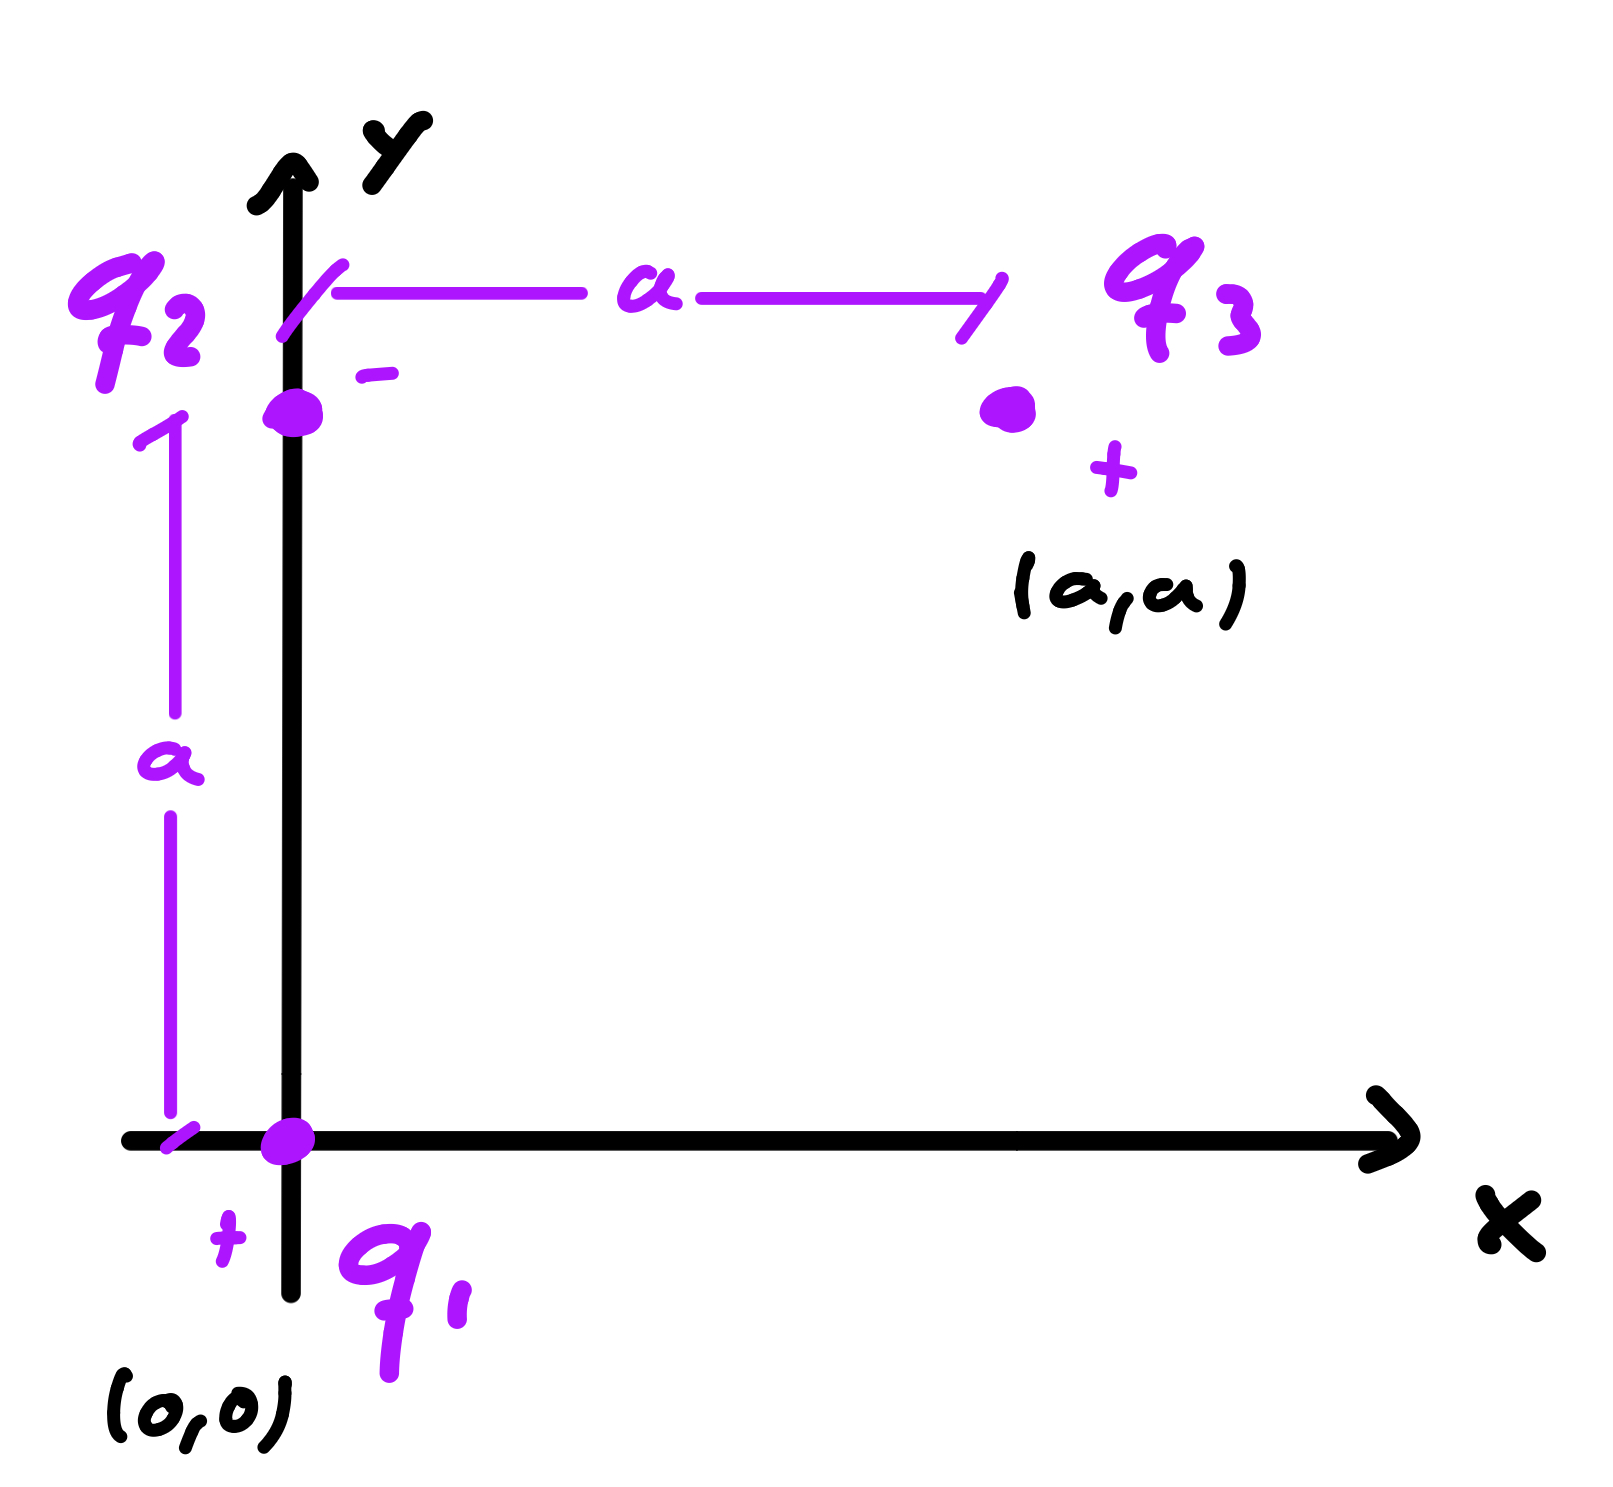
\includegraphics[width=0.35\textwidth]{imagen_1.jpeg}
  \caption{Descripción breve de la imagen.}
  \label{fig:imagen1}
\end{figure}
Determinar la $\vec{F}_e$ sobre $q_3$. \\
Atendiendo al principio de superposición tenemos:
\[
\vec{F}_e = \vec{F}_{q_2 q_3} + \vec{F}_{q_1 q_3}
\]
Aplicamos la ley de Coulomb:
\[
\vec{F}_{q_1 q_3} = \frac{1}{4\pi \varepsilon_0} \frac{q_1 q_3}{r_{13}^2} \, \hat{r}_{13}, 
\]
calculamos el vector unitario $\hat{r}_{13}$:
\[
\vec{r}_{13} = (2a,2a), 
\qquad r_{13} = \sqrt{(2a)^2+(2a)^2} = \sqrt{8a^2} = 2\sqrt{2}\,a
\]
\[
\hat{r}_{13} = \frac{\vec{r}_{13}}{|\vec{r}_{13}|} = \frac{2a\,\hat{\imath} + 2a\,\hat{\jmath}}{2\sqrt{2}\,a} 
= \frac{\sqrt{2}}{2} (\hat{\imath} + \hat{\jmath})
\]
Entonces:\\
\[
\vec{F}_{q_1 q_3} = \frac{1}{4\pi \varepsilon_0} \frac{q_1 q_3}{(2\sqrt{2}\,a)^2} \, \hat{r}_{13}
= \frac{1}{4\pi \varepsilon_0} \frac{q_1 q_3}{8a^2} \, \frac{\sqrt{2}}{2} (\hat{\imath} + \hat{\jmath})
\]
Vemos ahora $q_2 \to q_3$:\\
\[
\vec{F}_{q_2 q_3} = \frac{1}{4\pi \varepsilon_0} \frac{q_2 q_3}{r_{23}^2} \, \hat{r}_{23}, \\
\]
Calculamos el vector unitario $\hat{r}_{23}$:
\[
\vec{r}_{23} = (a,0), \qquad r_{23}=a, \qquad \hat{r}_{23} = \frac{\vec{r}_{23}}{|\vec{r}_{23}|} = \hat{\imath}
\]
Entonces:
\[
\vec{F}_{q_2 q_3} = \frac{1}{4\pi \varepsilon_0} \frac{q_2 q_3}{a^2} \, \hat{\imath}\\
\]
Por último calculamos la fuerza total en $q_3$ con el principio de superposición:
\[
\vec{F}_e = \vec{F}_{13} + \vec{F}_{23}
\]
\[
\vec{F}_e =
\frac{1}{4\pi\varepsilon_0}\,\frac{q_1 q_3}{2a^2}\,\frac{\sqrt{2}}{2}\,(\hat{\imath}+\hat{\jmath})
\;+\;
\frac{1}{4\pi\varepsilon_0}\,\frac{q_2 q_3}{a^2}\,\hat{\imath}
\;=\;
\frac{q_3}{4\pi\varepsilon_0}\!\left[
\left(\frac{q_2}{a^2}-\frac{q_1}{2a^2}\right)\hat{\imath}
+\frac{q_1}{2a^2}\hat{\jmath}
\right]
\]

\newpage

\section{Campos eléctricos}
\noindent
El \textbf{campo eléctrico} en un punto se define como la fuerza eléctrica por unidad de carga de prueba positiva colocada en ese punto:
\[
\vec E(\vec r) \;=\; \lim_{q_0 \to 0}\,\frac{\vec F_e(\vec r)}{q_0}.
\]

\subsection*{Derivación desde la ley de Coulomb}
\noindent
Para una carga puntual $q$ situada en $\vec r'$, la fuerza sobre una carga de prueba $q_0$ en $\vec r$ es
\[
\vec F_e \;=\; \frac{1}{4\pi\varepsilon_0}\,\frac{q\,q_0}{|\vec r-\vec r'|^2}\,\hat{\mathbf R},
\qquad \hat{\mathbf R}=\frac{\vec r-\vec r'}{|\vec r-\vec r'|}.
\]
Dividiendo por $q_0$, queda:
\[
\boxed{\;\vec E(\vec r)\;=\;\frac{1}{4\pi\varepsilon_0}\,\frac{q}{|\vec r-\vec r'|^2}\,\hat{\mathbf R}\;}
\]
y, en el caso de tomar el origen en la carga y $r=|\vec r|$,
\[
\vec E_q \;=\; \frac{1}{4\pi\varepsilon_0}\,\frac{q}{r^2}\,\hat r .
\]
%%% Figura 2 %%%
\begin{center}
\begin{tikzpicture}[scale=1]
% Carga positiva (sale)
\begin{scope}
  \filldraw (0,0) circle (2pt);
  \foreach \a in {0,30,...,330}{
    \draw[-{Latex}] (0,0) -- ({1.6*cos(\a)},{1.6*sin(\a)});
  }
  \node[below] at (0,-1.9) {\small \textit{Diverge}};
\end{scope}
% Carga negativa (entra)
\begin{scope}[xshift=4.5cm]
  \filldraw (0,0) circle (2pt);
  \foreach \a in {0,30,...,330}{
    \draw[-{Latex}] ({1.6*cos(\a)},{1.6*sin(\a)}) -- (0,0);
  }
  \node[below] at (0,-1.9) {\small \textit{Lo succiona}};
\end{scope}
\end{tikzpicture}
\end{center}

\[
\vec E_q \;=\; \frac{1}{4\pi\varepsilon_0}\,\frac{q}{r^2}\,\hat r_{qP}
\]

\newpage

\subsection*{Distribuciones de carga}
Pueden ser:
\[
\text{Lineales} \;\Rightarrow\; \lambda \;=\; \frac{dq}{dl},
\qquad
\text{Superficiales} \;\Rightarrow\; \sigma \;=\; \frac{dq}{dA},
\qquad
\text{Volumétrica} \;\Rightarrow\; \rho \;=\; \frac{dq}{dV}.
\]
%%% Figura 3 %%%
\vspace{-2.0em}
\begin{figure}[h]
  \centering
  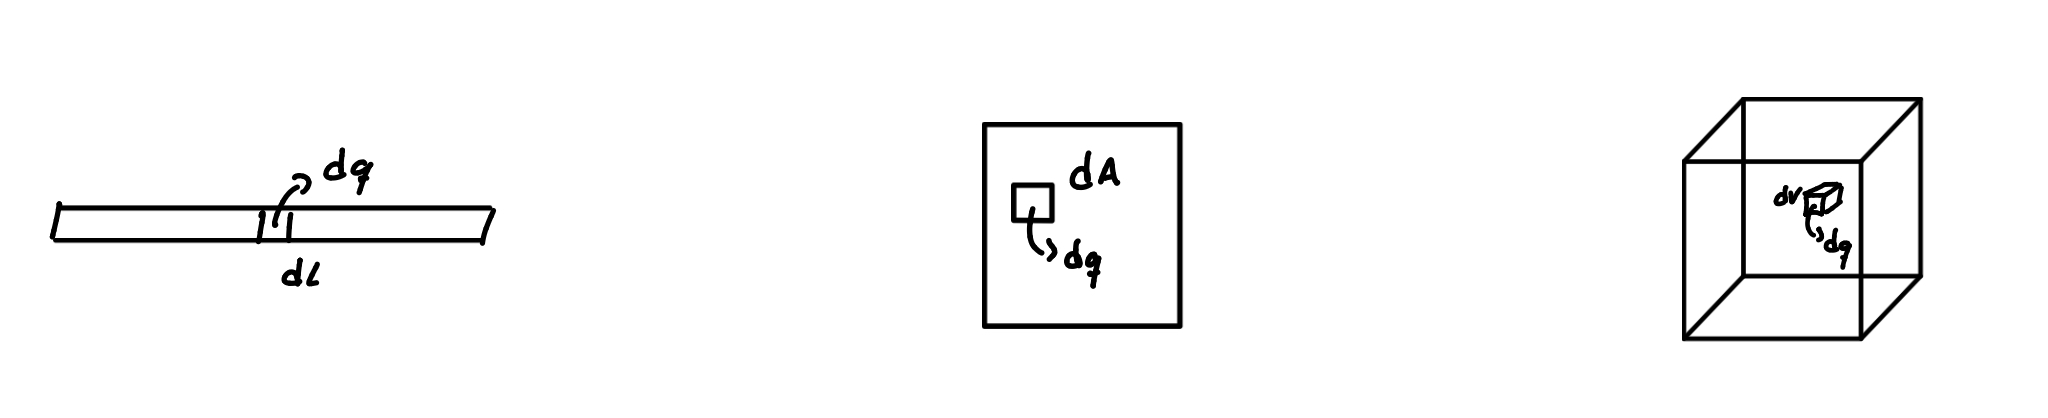
\includegraphics[width=1.0\textwidth]{imagen_2.jpeg}
  \caption{Descripción breve de la imagen.}
  \label{fig:imagen2}
\end{figure}

\subsection*{Ejemplo:}
\noindent
Tenemos una barra de longitud $l$ con una distribución de carga lineal homogénea $\lambda$.
Determine el campo eléctrico generado por la barra a una distancia $d$ de uno de sus extremos.
¿Qué ocurre cuando $d \gg l$?

%%% Figura 4 %%%
\begin{figure}[h]
  \centering
  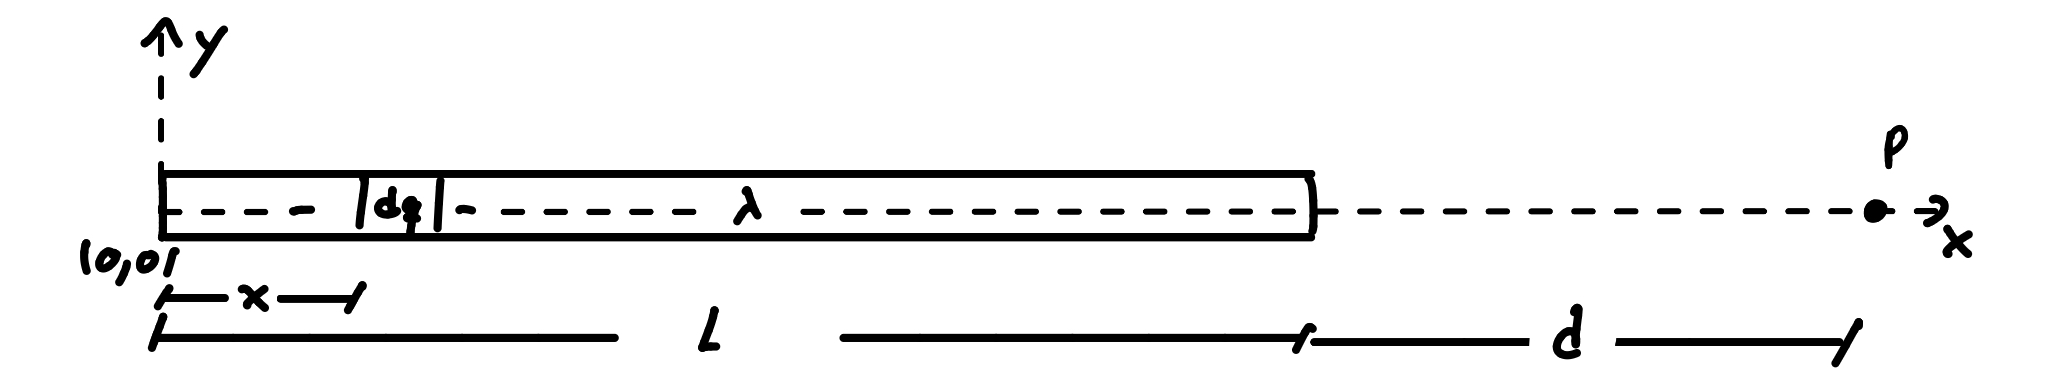
\includegraphics[width=0.8\textwidth]{imagen_3.jpeg}
  \caption{Descripción breve de la imagen.}
  \label{fig:imagen3}
\end{figure}
Planteamos la solución del campo eléctrico
\[
\vec E \;=\; \frac{1}{4\pi\varepsilon_0}\int \frac{dq}{r^2}\,\hat r_{qP},
\qquad
\]
Siendo el vector unitario $\hat{r}_{qP}$:
\[
\hat r_{qP} \;=\; \frac{\vec r_P-\vec r_q}{\lvert \vec r_P-\vec r_q\rvert}
\;=\; \frac{(l+d)\,\hat{\imath}-x\,\hat{\imath}}{\lvert (l+d)-x\rvert}
\; \hat{\imath}
\]
Donde:
\[
r^2 = \bigl((l+d)-x\bigr)^2,
\qquad
dq = \lambda\,dl = \lambda\,dx.
\]
Entonces:
\[
\vec E \;=\; \frac{1}{4\pi\varepsilon_0}\int_{0}^{l}
\frac{\lambda\,dx}{\bigl((l+d)-x\bigr)^2}\,\hat{\imath}
\;=\;
\frac{\lambda}{4\pi\varepsilon_0}\left[ -\,\frac{1}{(l+d)-x} \right]_{0}^{l}\hat{\imath}
\;=\;
\frac{\lambda}{4\pi\varepsilon_0}\!\left(\frac{1}{d}-\frac{1}{l+d}\right)\hat{\imath}.
\]

\paragraph*{(b) $d\gg l$}
\[
\vec E \;\approx\; \frac{\lambda}{4\pi\varepsilon_0}\left(\frac{l}{d(l+d)}\right)\hat{\imath}
\;\approx\; \frac{\lambda\,l}{4\pi\varepsilon_0\,d^{2}}\,\hat{\imath}
\;\approx\; \frac{Q}{4\pi\varepsilon_0\,d^{2}}\,\hat{\imath}
\quad\text{con } Q=\lambda\,l.
\]
Llegamos a la expresión del campo eléctrico de una carga puntual $Q$. ya que al estar tan alejados la barra se comporta como una carga puntual.

\newpage

\subsection*{Ejemplo:}

Calcular $\vec E$ en el punto $P$.  
¿Qué ocurre si $P \gg L$?

%%% Figura 5 %%%
\begin{figure}[h]
  \centering
  \includegraphics[width=0.5\textwidth]{imagen_4.jpeg}
  \caption{Descripción breve de la imagen.}
  \label{fig:imagen4}
\end{figure}

\noindent Pista: 

\[
\int \frac{y}{(x^2+y^2)^{3/2}}\,dx \;=\; \frac{x}{y\sqrt{x^2+y^2}}
\]
La solución del campo será:

\[
\vec E = \frac{1}{4\pi\varepsilon_0} \int \frac{dq}{r^2}\,\hat r_{qP},
\qquad
\hat r_{qP} = \frac{\vec r_P-\vec r_q}{|\vec r_P-\vec r_q|}
= \frac{-x}{\sqrt{x^2+y^2}}\,\hat{\imath} + \frac{y}{\sqrt{x^2+y^2}}\,\hat{\jmath}.
\]
Sustituyendo:
\[
\vec E = \frac{1}{4\pi\varepsilon_0} \int_{-L/2}^{L/2}
\frac{\lambda\,dx}{(x^2+y^2)}\,
\left( -\frac{x}{\sqrt{x^2+y^2}}\,\hat{\imath}
+ \frac{y}{\sqrt{x^2+y^2}}\,\hat{\jmath} \right)
\]
Al tratarse de una integral vectorial, se integra cada componente por separado:

\[
\vec E =
\frac{\lambda}{4\pi\varepsilon_0} \left[
\int_{-L/2}^{L/2} \frac{-x}{(x^2+y^2)^{3/2}}\,dx \;\hat{\imath}
+ \int_{-L/2}^{L/2} \frac{y}{(x^2+y^2)^{3/2}}\,dx \;\hat{\jmath}
\right]
\]

\[
= \frac{\lambda}{4\pi\varepsilon_0} \left[
\left. -\frac{1}{\sqrt{x^2+y^2}} \right|_{-L/2}^{L/2} \hat{\imath}
+ \left. \frac{x}{y\sqrt{x^2+y^2}} \right|_{-L/2}^{L/2} \hat{\jmath}
\right]
\]


\newpage
\subsection{Coordenadas cilíndricas}

\noindent Las \textbf{coordenadas cilíndricas} representan un punto en el espacio mediante la tripleta
 $(r,\theta,z)$, donde $r$ es la distancia desde el punto al eje $z$ (coordenada radial),
  $\theta$ es el ángulo que forma el radio con el eje $x$ (coordenada acimutal) y $z$ es la
   altura del punto sobre el plano $xy$ (coordenada vertical). Este sistema es una generalización
    de las coordenadas polares al espacio tridimensional y es útil en problemas con simetría cilíndrica.\\

\noindent Siendo las nuevas coordenadas:
\[
x = r\cos\theta, \quad y = r\sin\theta, \quad z = z
\]
%%% Figura 6 %%%
\vspace{-2.0em}
\begin{figure}[h]
  \centering
  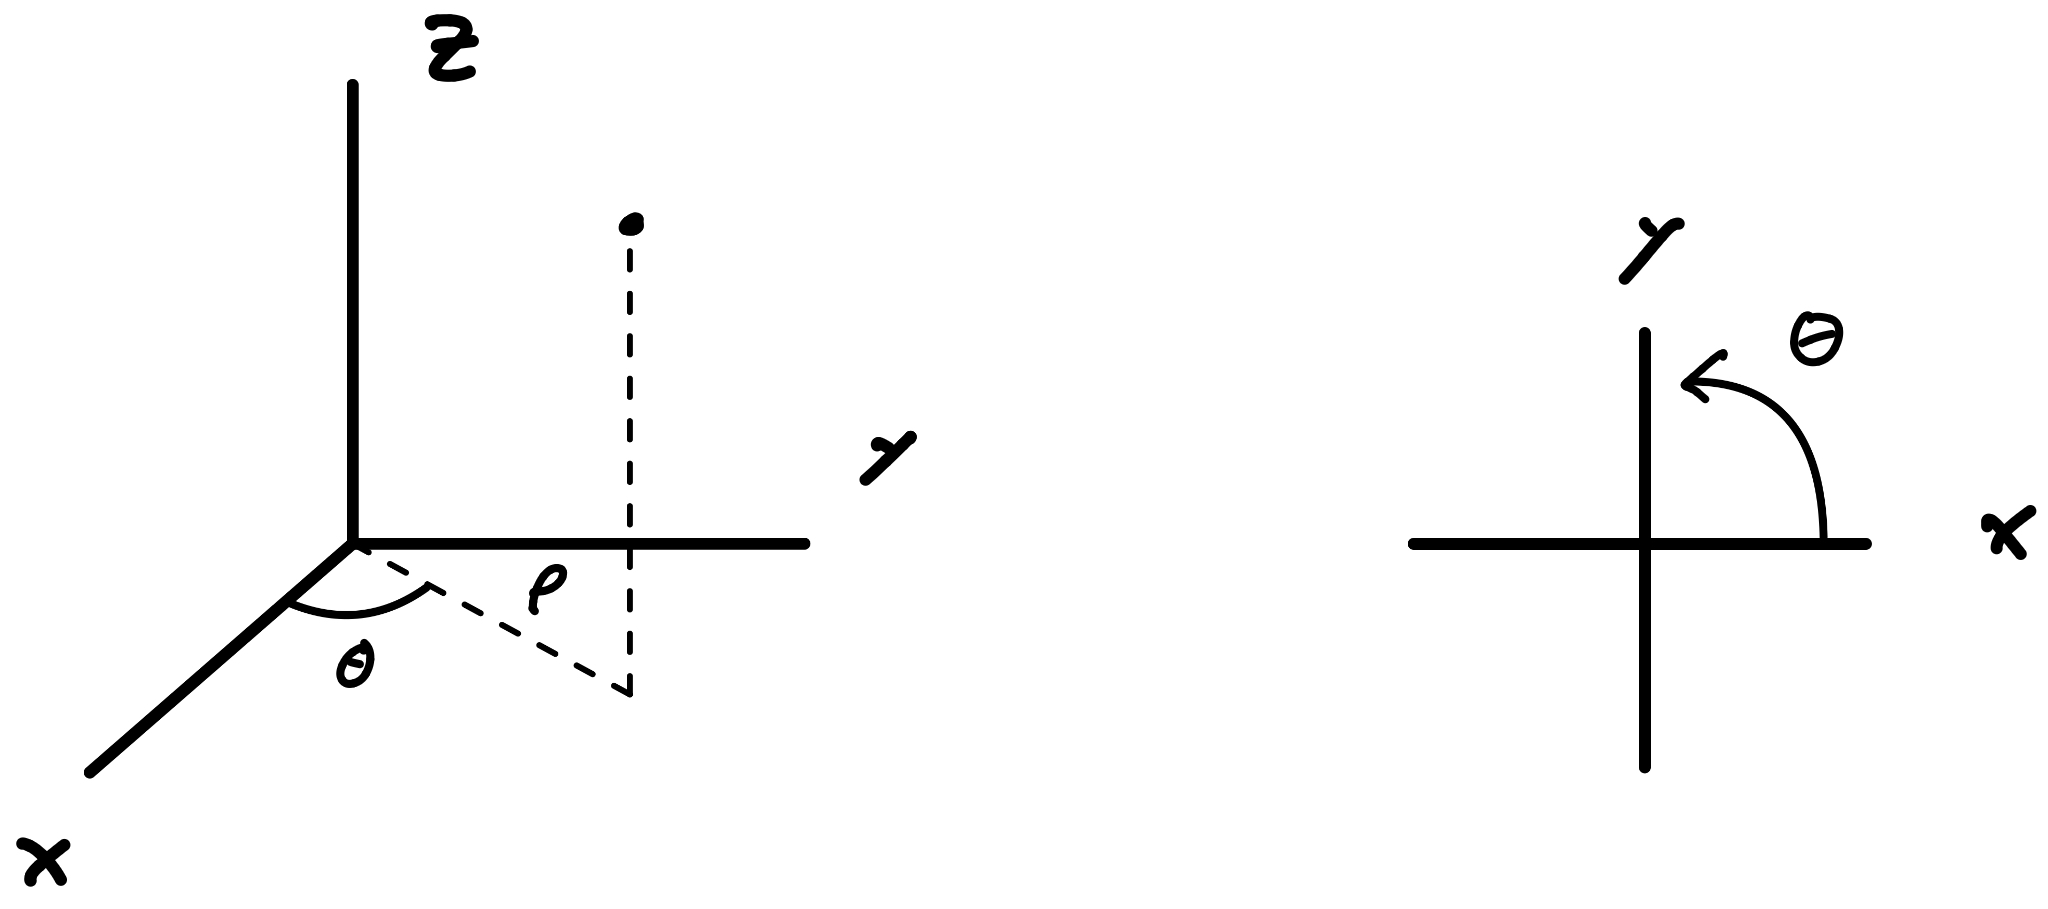
\includegraphics[width=0.65\textwidth]{imagen_5.jpeg}
  \caption{Descripción breve de la imagen.}
  \label{fig:imagen5}
\end{figure}

  % tus fórmulas...
Donde $\theta$ va siempre desde el eje positivo de $x$ al eje positivo de $y$.
Al igual que en coordenadas cartesianas, las coordenadas cilíndricas también tienen \textit{vectores unitarios}:
\[
\hat{\mathbf e}_r = \cos\theta\,\hat{\imath} + \sin\theta\,\hat{\jmath},\qquad
\hat{\mathbf e}_\theta = -\sin\theta\,\hat{\imath} + \cos\theta\,\hat{\jmath},\qquad
\hat{\mathbf e}_z = \hat{\mathbf k}.
\]
%%% figura 7 %%%
\vspace{-2.0em}
\begin{figure}[h]
  \centering
  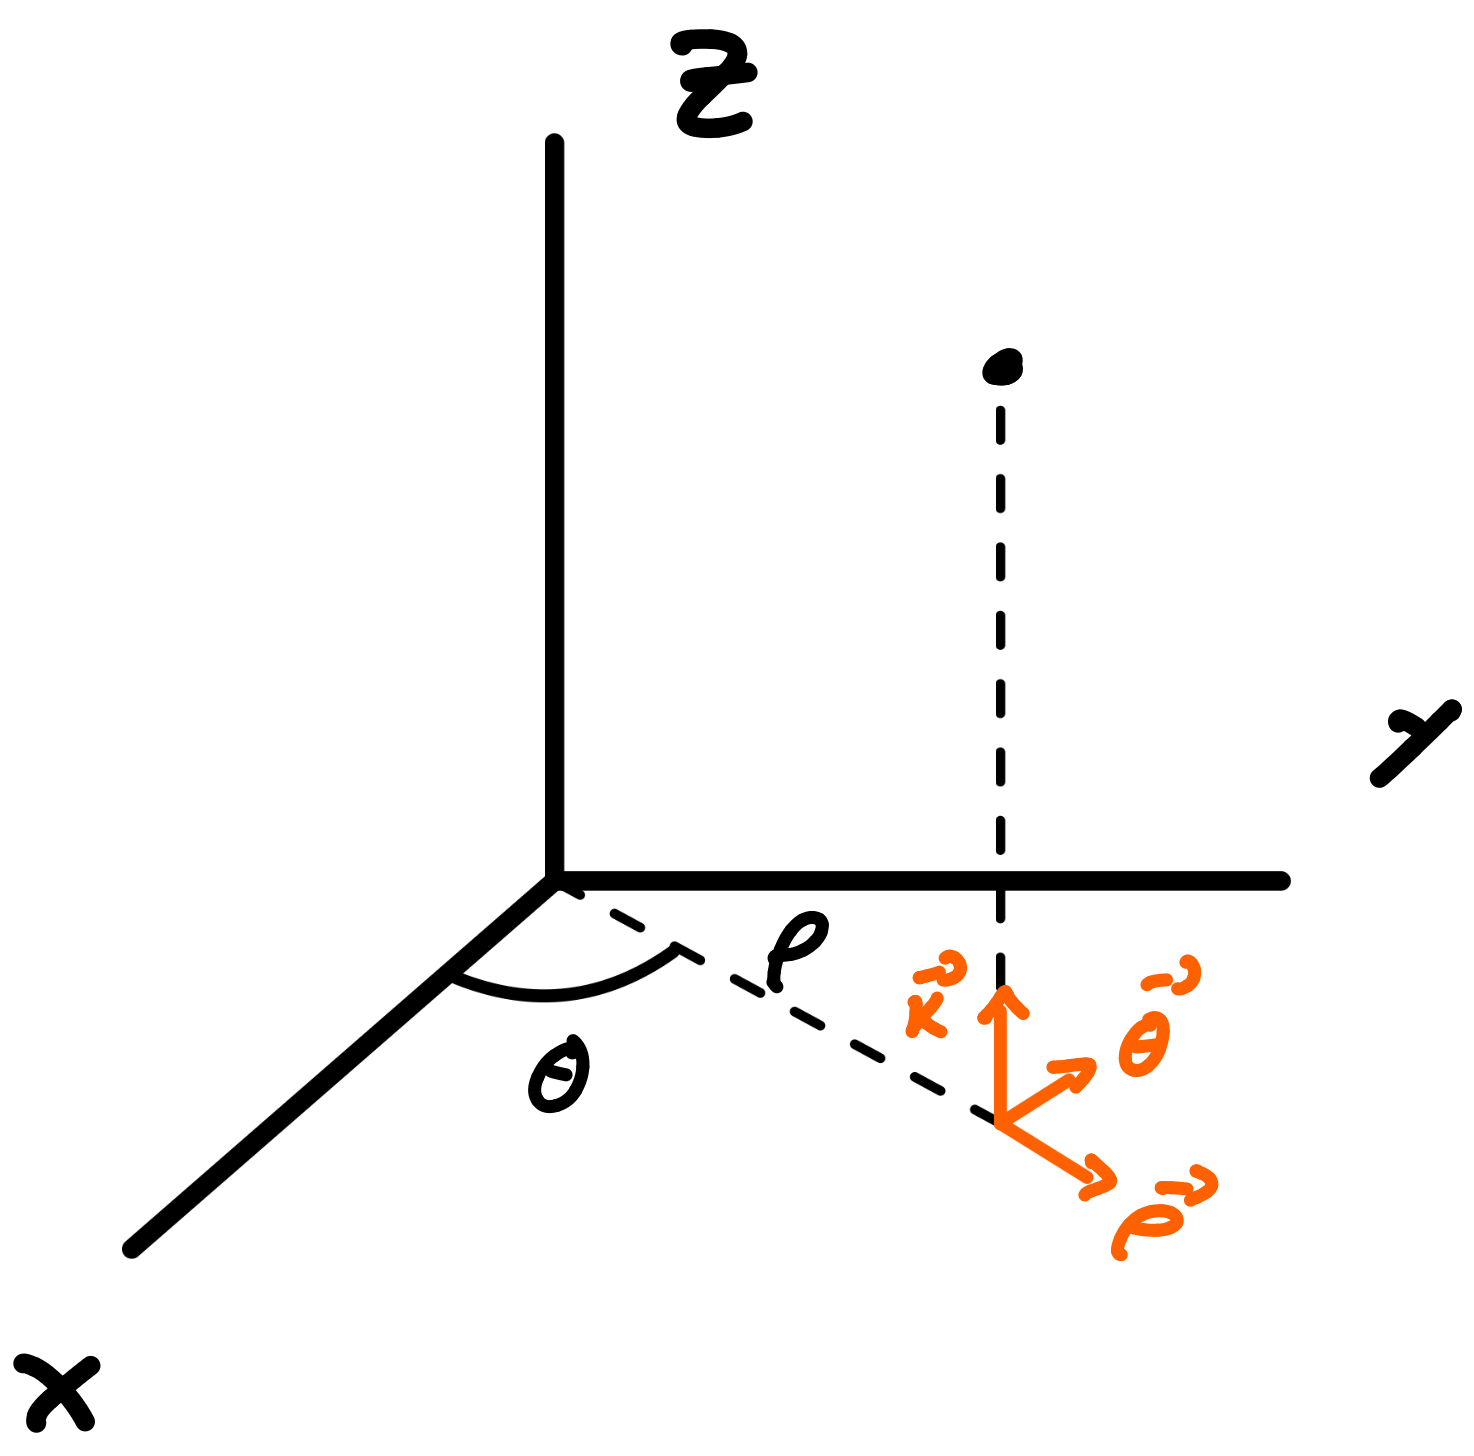
\includegraphics[width=0.3\textwidth]{imagen_6.jpeg}
  \caption{Descripción breve de la imagen.}
  \label{fig:imagen6}
\end{figure}
\newpage

\subsection{Diferenciales de longitud, área y volumen (cartesianas)}

De longitud:
\[
d\vec{\ell} = dx\,\hat{\imath} + dy\,\hat{\jmath} + dz\,\hat{\mathbf k}
\]

De área:
\[
\begin{aligned}
d\vec{A}_x &= dy\,dz\,\hat{\imath},\\
d\vec{A}_y &= dx\,dz\,\hat{\jmath},\\
d\vec{A}_z &= dx\,dy\,\hat{\mathbf k}.
\end{aligned}
\]

De volumen:
\[
dV = dx\,dy\,dz
\]

\textit{Hacer esquemas visuales.}


\subsection{Diferenciales de longitud, área y volumen (cilíndricas)}

De longitud:
\[
d\vec{\ell} = dr\,\hat{\mathbf e}_r + r\,d\theta\,\hat{\mathbf e}_\theta + dz\,\hat{\mathbf e}_z
\]

De área:
\[
\begin{aligned}
d\vec{S}_r      &= r\,d\theta\,dz\,\hat{\mathbf e}_r,\\
d\vec{S}_\theta &= dr\,dz\,\hat{\mathbf e}_\theta,\\
d\vec{S}_z      &= r\,dr\,d\theta\,\hat{\mathbf e}_z.
\end{aligned}
\]

De volumen:
\[
dV = r\,dr\,d\theta\,dz
\]
%%% Figura 8 %%%
\vspace{-2.0em}
\begin{figure}[h]
  \centering
  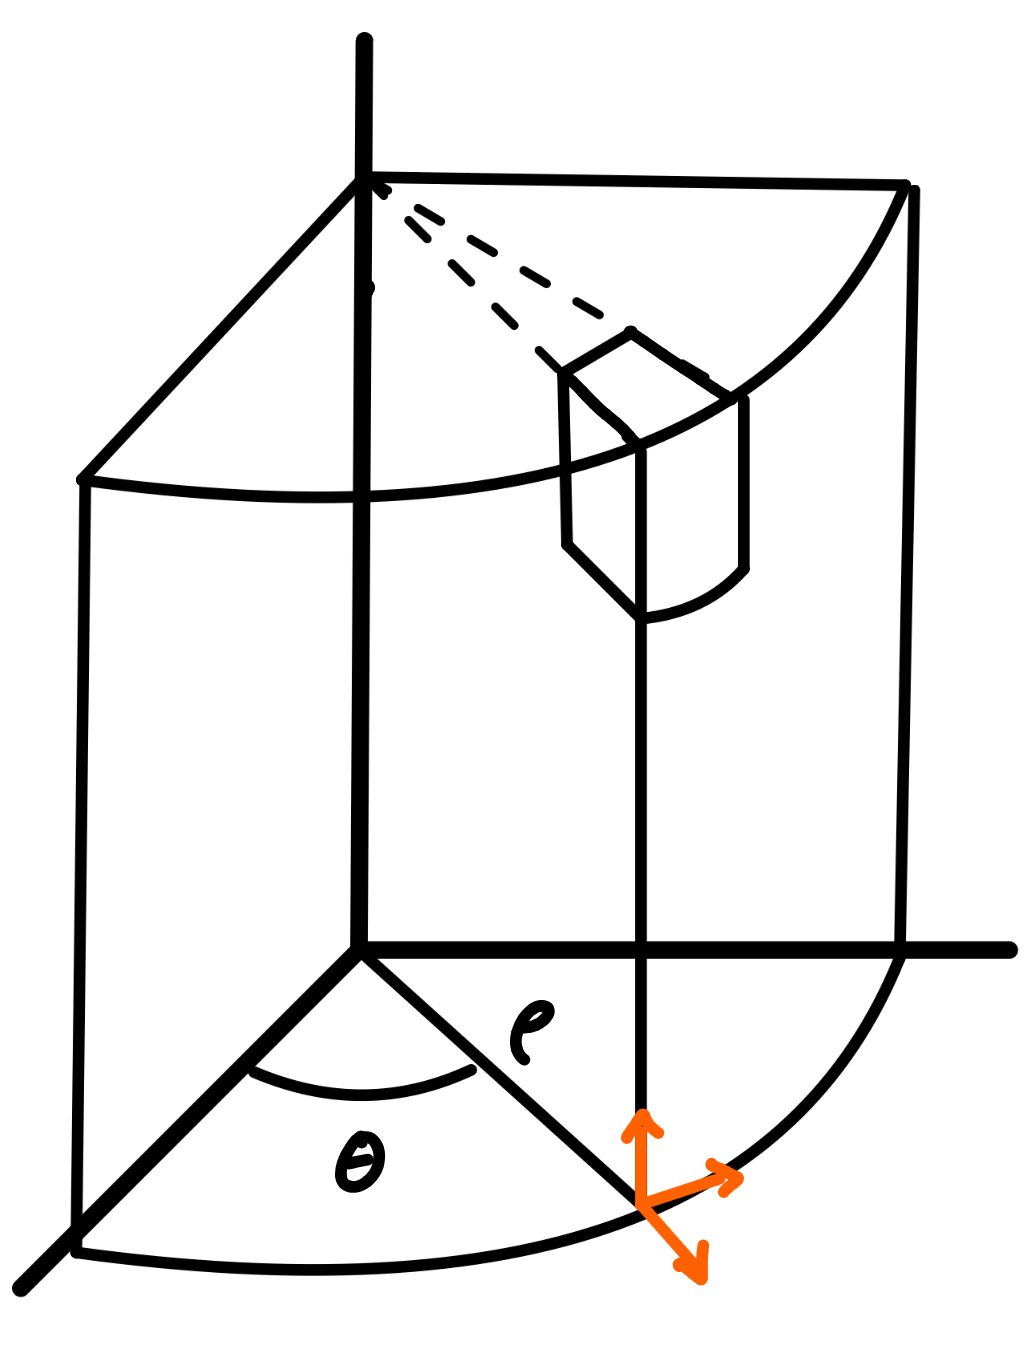
\includegraphics[width=0.25\textwidth]{imagen_7.jpeg}
  \caption{Descripción breve de la imagen.}
  \label{fig:imagen7}
\end{figure}


\subsection*{Ejemplo:}
\noindent Un anillo cargado con densidad de carga lineal variable $\lambda=\cos^{2}\theta$ y radio $a$.
Determinar la carga total.

La densidad lineal, por tanto la carga vendrá dada como:
\[
q_T \;=\; \oint \lambda\, dl
 \;=\; \int_{0}^{2\pi} \lambda\, a\, d\theta
 \;=\; a \int_{0}^{2\pi} \cos^{2}\theta\, d\theta .
\]

\textit{* Los límites de integración varían dependiendo de nuestro sistema de referencia.  
En nuestro caso $r=a$ y $\theta\in[0,2\pi]$.}


\subsection*{Ejemplo:}

\noindent
Un disco cargado con densidad de carga superficial $\sigma=\rho\,\sin^{2}\theta$ y radio $R$.  
Determina la \textbf{carga total} del disco.

\[
q_T \;=\; \iint_{S} \sigma\, dA
   \;=\; \int_{0}^{2\pi}\!\left(\int_{0}^{R} \rho\,\sin^{2}\theta \; r\,dr\right)\! d\theta .
\]

\subsection*{Ejemplo:}
\noindent
Un anillo cargado con densidad de carga lineal constante $\lambda$ y radio $a$.  
Determine el valor del \textbf{campo eléctrico} en el punto $P$ (sobre el eje del anillo, a altura $z$).
\[
\vec E
= \frac{1}{4\pi\varepsilon_0}\oint \frac{dq}{r^2}\,\hat r
= \frac{1}{4\pi\varepsilon_0}\int_{0}^{2\pi}
   \frac{\lambda a\, d\theta}{a^{2}+z^{2}}\;
   \frac{-a\cos\theta\,\hat{\imath}\;-\;a\sin\theta\,\hat{\jmath}\;+\;z\,\hat{\mathbf k}}
        {\sqrt{a^{2}+z^{2}}}.
\]
Como integral vectorial, se integran las componentes por separado:
\[
\int_{0}^{2\pi} \frac{-a\cos\theta}{(a^{2}+z^{2})^{3/2}}\, d\theta = 0, \qquad
\int_{0}^{2\pi} \frac{-a\sin\theta}{(a^{2}+z^{2})^{3/2}}\, d\theta = 0,
\]
\[
\int_{0}^{2\pi} \frac{z}{(a^{2}+z^{2})^{3/2}}\, d\theta
= \frac{2\pi z}{(a^{2}+z^{2})^{3/2}}.
\]
Por tanto,
\[
\boxed{\;
\vec E(P) \;=\; \frac{\lambda a z}{2\,\varepsilon_0\,(a^{2}+z^{2})^{3/2}}\;\hat{\mathbf k}
\;}
\]
\newpage
\subsection{Coordenadas esféricas}
\noindent Las \textbf{coordenadas cilíndricas} representan un punto en el espacio mediante la tripleta
 $(r,\theta,\phi)$, donde $r$ es la distancia desde el punto al origen (coordenada radial),
  $\theta$ es el ángulo que forma el radio con el eje $x$ (coordenada acimutal) y $\phi$ es el
   ángulo que forma el radio con el eje $z$ (coordenada polar). Este sistema es una generalización
    de las coordenadas polares al espacio tridimensional y es útil en problemas con simetría esférica.\\

\noindent Siendo las nuevas coordenadas:
\[
x = r\sin\theta\cos\phi, \quad y = r\sin\theta\sin\phi, \quad z = r\cos\theta
\]
\vspace{-2.0em}
\begin{figure}[htbp]
  \centering
  % Si renombraste el archivo:
  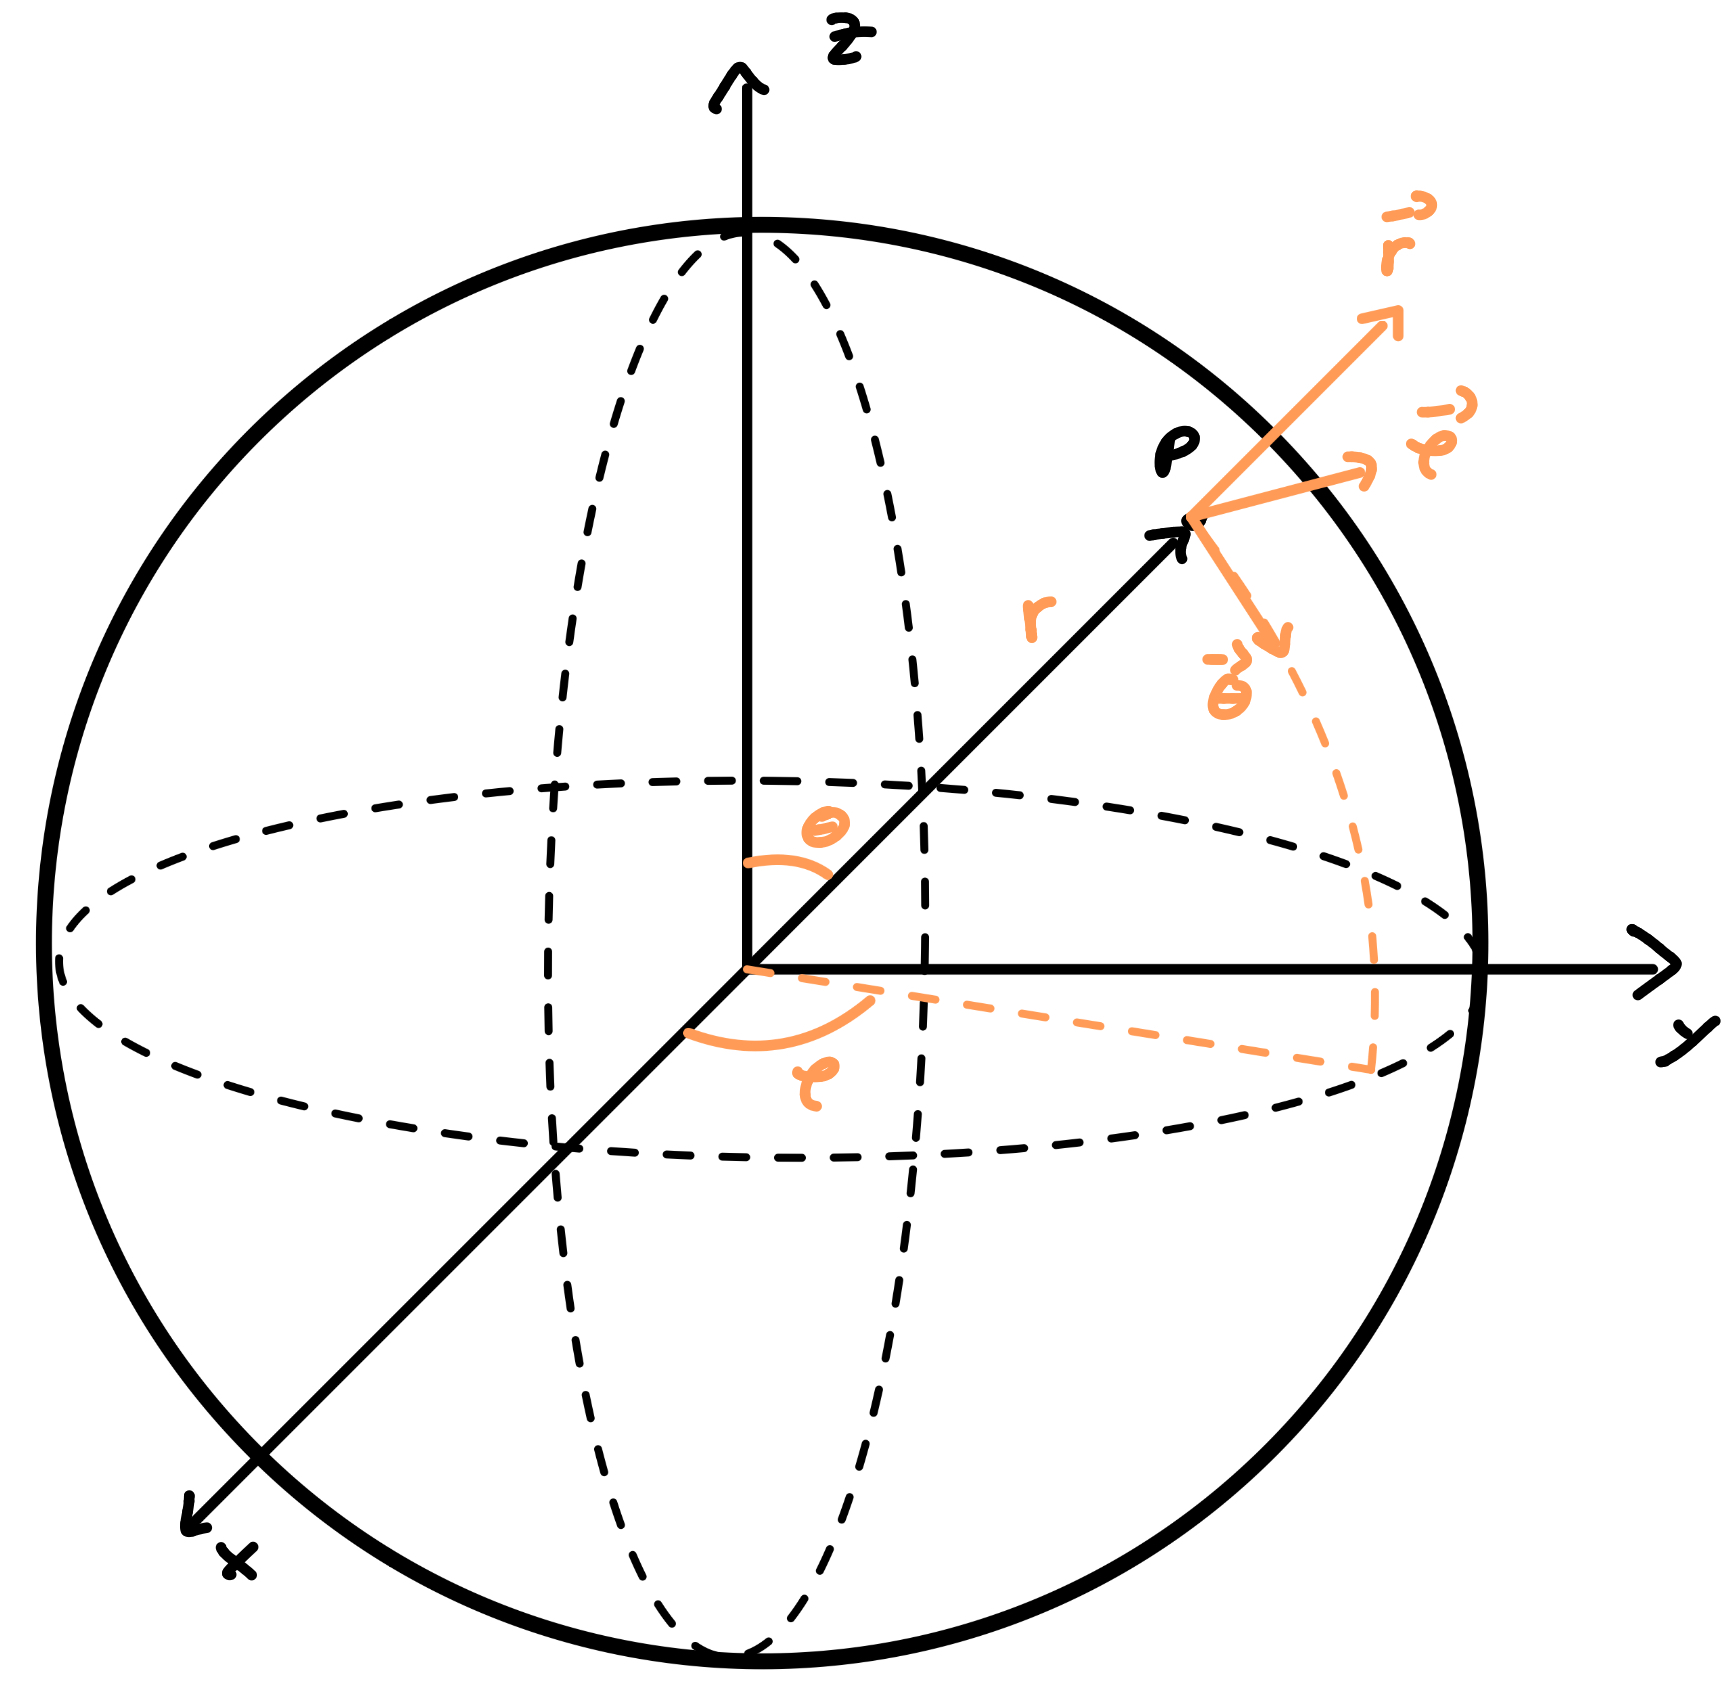
\includegraphics[width=0.40\textwidth]{esfericas.jpg}
  % O si mantienes el nombre con espacios:
  % \includegraphics[width=0.82\textwidth]{Esquemas\ Y\ Dibujos.jpeg}
  \caption{Coordenadas esféricas: $r$, $\theta$, $\varphi$.}
  \label{fig:esfericas}
\end{figure}

\subsection*{Diferenciales de longitud, área y volumen (esféricas)}

De longitud:
\[
d\vec{\ell} = dr\,\hat{\mathbf e}_r + r\,d\theta\,\hat{\mathbf e}_\theta + r\sin\theta\,d\phi\,\hat{\mathbf e}_\phi
\]

De área:
\[
\begin{aligned}
d\vec{S}_r      &= r^{2}\sin\theta\,d\theta\,d\phi\,\hat{\mathbf e}_r, \\
d\vec{S}_\theta &= r\sin\theta\,dr\,d\phi\,\hat{\mathbf e}_\theta, \\
d\vec{S}_\phi   &= r\,dr\,d\theta\,\hat{\mathbf e}_\phi.
\end{aligned}
\]

De volumen:
\[
dV = r^{2}\sin\theta\,dr\,d\theta\,d\phi
\]

\subsection*{Ejemplo:}
\noindent
Una esfera de radio $r$ tiene una densidad superficial dada como:

\[
\sigma = x^{2} + y^{2} + z^{2}
\]
Determina su carga total:

\[
Q_T = \int_{A} \sigma\, dA
\]
donde:

\[
dA = r^{2}\sin\theta\, d\theta\, d\phi
\]

\[
Q_T = \int_{0}^{2\pi}\int_{0}^{\pi} r^{2}\sin\theta\, d\theta\, d\phi = 4\pi r^{4}
\]
\subsection*{Ejemplo:}
\[
V = \int_{V} dV = \int_{0}^{2\pi}\int_{0}^{\pi}\int_{0}^{r} r^{2}\sin\theta\, d\phi\, d\theta\, dr
\]\\
Una esfera de radio $R$ tiene una densidad de carga volumétrica de 
\[
\rho = e^{(x^{2}+y^{2}+z^{2})^{1/2}} = e^{r}
\]
Determina la carga total:

\[
Q_T = \int_{V} \rho\, dV = \int_{0}^{2\pi}\int_{0}^{\pi}\int_{0}^{R} e^{r} r^{2}\sin\theta\, dr\, d\theta\, d\phi
\]\\
\[
Q_T = 4\pi \int_{0}^{R} e^{r} r^{2}\, dr = \frac{4\pi}{3}\left(e^{R} - 1\right)
\]
\newpage
\noindent
\subsection*{Ejemplo:}
\noindent 
Determina el campo eléctrico que genera una carga puntual en cualquier punto del espacio.

\textbf{a) Con coordenadas cartesianas}
\[
\vec E \;=\; \frac{1}{4\pi\varepsilon_0}\,\frac{q}{r_q^{\,2}}\;\hat r_q
\]

Calculamos el vector unitario $\hat r_q$:
\[
\hat r_q \;=\; \frac{\vec r_P-\vec r_q}{\lvert \vec r_P-\vec r_q\rvert}
= \frac{x\,\hat{\imath}+y\,\hat{\jmath}+z\,\hat{\mathbf k}-0}{\sqrt{x^{2}+y^{2}+z^{2}}}
\]

La añadimos a la expresión del campo:
\[
\vec E \;=\; \frac{1}{4\pi\varepsilon_0}\;
\frac{q}{x^{2}+y^{2}+z^{2}}\;
\frac{x\,\hat{\imath}+y\,\hat{\jmath}+z\,\hat{\mathbf k}}{\sqrt{x^{2}+y^{2}+z^{2}}}
= \frac{1}{4\pi\varepsilon_0}\;
\frac{q\,(x\,\hat{\imath}+y\,\hat{\jmath}+z\,\hat{\mathbf k})}{(x^{2}+y^{2}+z^{2})^{3/2}}.
\]\\

\textbf{b) Con coordenadas cilíndricas}
\[
\vec E \;=\; \frac{1}{4\pi\varepsilon_0}\,\frac{q}{r_q^{\,2}}\;\hat r_q
\]

Calculamos el vector unitario $\hat r_q$:
\[
\hat r_q \;=\; \frac{\vec r_P-\vec r_q}{\lvert \vec r_P-\vec r_q\rvert}
= \frac{\rho\,\hat{\mathbf e}_\rho + z\,\hat{\mathbf k}-0}{\sqrt{\rho^{2}+z^{2}}}
\]

La añadimos a la expresión del campo:
\[
\vec E \;=\; \frac{1}{4\pi\varepsilon_0}\;
\frac{q}{\rho^{2}+z^{2}}\;
\frac{\rho\,\hat{\mathbf e}_\rho + z\,\hat{\mathbf k}}{\sqrt{\rho^{2}+z^{2}}}
= \frac{1}{4\pi\varepsilon_0}\;
\frac{q\left(\rho\,\hat{\mathbf e}_\rho + z\,\hat{\mathbf k}\right)}{(\rho^{2}+z^{2})^{3/2}}.
\]\\

\textbf{c) Con coordenadas esféricas}
\[
\vec E \;=\; \frac{1}{4\pi\varepsilon_0}\,\frac{q}{r_q^{\,2}}\;\hat r_q
\]

Calculamos el vector unitario $\hat r_q$:
\[
\hat r_q \;=\; \frac{\vec r_P-\vec r_q}{\lvert \vec r_P-\vec r_q\rvert}
= \frac{r\,\hat{\mathbf e}_r - 0}{r} \;=\; \hat{\mathbf e}_r
\]

La añadimos a la expresión del campo:
\[
\vec E \;=\; \frac{1}{4\pi\varepsilon_0}\,\frac{q}{r^{2}}\;\hat{\mathbf e}_r .
\]
\newpage
\noindent
\textbf{Ejercicio 2:} Un cilindro de radio \(R\) tiene su superficie circular cargada con una densidad de carga constante.
Determina el campo eléctrico generado a una distancia \(d\) de su eje como muestra la figura.

\medskip
\noindent
El campo eléctrico generado por el cilindro vendrá dado como:
\[
\vec E \;=\; \frac{1}{4\pi\varepsilon_0}\iint \frac{dq}{r^{2}}\;\hat r_{qP}.
\]
Con elemento de carga superficial
\[
dq=\sigma\,dA=\sigma\,R\,d\theta\,dz;
\qquad
\theta\in[0,2\pi],\;\; z\in[0,h].
\]
Calculamos el vector
\[
\vec r_{qP}=\vec r_P-\vec r_q
= (h+d)\,\hat{\mathbf k} - \big(R\,\hat{\mathbf e}_r + z\,\hat{\mathbf k}\big),
\]
\[
|\vec r_{qP}|=\sqrt{R^{2}+(h+d-z)^{2}}.
\]
Sustituyendo:
\[
\vec E
=\frac{\sigma R}{4\pi\varepsilon_0}
\int_{0}^{h}\!\!\int_{0}^{2\pi}
\left[
\frac{-\,R\,\hat{\mathbf e}_r}{\big(R^{2}+(h+d-z)^{2}\big)^{3/2}}
+\frac{(h+d-z)\,\hat{\mathbf k}}{\big(R^{2}+(h+d-z)^{2}\big)^{3/2}}
\right] d\theta\,dz .
\]

\textit{Nota:} hay que cambiar \(\hat{\mathbf e}_r\) por \(\cos\theta\,\hat{\imath}+\sin\theta\,\hat{\jmath}\) ya que \(\hat{\mathbf e}_r\) depende de \(\theta\).

\bigskip
\noindent
\textbf{Ejercicio 3.}
Un recipiente hemisférico de radio \(a\) tiene una carga total \(q\) repartida uniformemente en su superficie.
Encuentre el campo eléctrico en el centro de curvatura (véase la figura).

\medskip
\noindent
El campo eléctrico viene dado como
\[
\vec E \;=\; \frac{1}{4\pi\varepsilon_0}\,\int \frac{dq}{r^{2}}\;\hat r .
\]
\textbf{Sustituimos.} Como por simetría sólo queda la componente sobre el eje,
\[
E_z \;=\; \frac{1}{4\pi\varepsilon_0}
\int_{0}^{2\pi}\!\!\int_{0}^{\pi/2}
\frac{dq}{a^{2}}\;\cos\theta ,
\quad
dq=\sigma\,dA,\quad
dA=a^{2}\sin\theta\,d\theta\,d\varphi,
\quad
\sigma=\frac{q}{2\pi a^{2}} .
\]
Por tanto:
\[
E_z \;=\; \frac{1}{4\pi\varepsilon_0}
\int_{0}^{2\pi}\!\!\int_{0}^{\pi/2}
\frac{\sigma a^{2}\sin\theta\,d\theta\,d\varphi}{a^{2}}\;\cos\theta .
\]
Además,
\[
\hat r_{qP}\;=\;\frac{\vec r_{P}-\vec r_{q}}{\lvert \vec r_{P}-\vec r_{q}\rvert},
\qquad
\lvert \vec r_{P}-\vec r_{q}\rvert = a .
\]

\bigskip
\subsection{Ley de Gauss}
\noindent
La ley de Gauss en electrostática relaciona el flujo de campo eléctrico a través de una
superficie cerrada con la carga neta encerrada en ella, afirmando que el flujo es igual
a la carga neta dividida por la permitividad del vacío. Matemáticamente, se expresa como:
\[
\oint_{\partial V}\vec E\cdot d\vec A \;=\; \frac{q_{\text{enc}}}{\varepsilon_0}.
\]\\
La ley de Gauss proviene de la primera ley de Maxwell; para llegar a ella partimos del
\emph{teorema de la divergencia}:
\[
\oint_{\partial V}\vec E\cdot d\vec A
\;=\;
\iiint_{V} (\nabla\!\cdot\!\vec E)\,dV,
\]
\[
\frac{q_{\text{enc}}}{\varepsilon_0}
=
\iiint_{V} \frac{\rho}{\varepsilon_0}\,dV
\]
\[
\nabla\!\cdot\!\vec E \;=\; \frac{\rho}{\varepsilon_0}
\quad\text{(primera ley de Maxwell en el vacío).}
\]
Si hay divergencia en el campo, es decir, \(\nabla\!\cdot\!\vec E>0\), el campo \emph{diverge} (fuente).
Si por el contrario \(\nabla\!\cdot\!\vec E<0\), tenemos un \emph{sumidero}, es decir, el campo \emph{converge}.\\

\noindent
Para usar la \textbf{ley de Gauss} tengo que crear una \textbf{superficie imaginaria} a mi conveniencia para poder integrar sobre ella.
\subsection*{Ejemplo:}
\noindent 
Se tiene una esfera aislante con una distribución de carga homogénea repartida uniformemente en su volumen.  
La esfera tiene radio \(R\). Determina el campo eléctrico producido por la esfera en todo el espacio.

\medskip
\noindent
Primero calculamos el campo \textbf{fuera de la esfera} (\(r > R\)).  
Para ello, mi \textbf{superficie gaussiana} será una esfera concéntrica de radio \(r\).

\[
\oint_{\partial V}\vec E\cdot d\vec A = \frac{q_{\text{enc}}}{\varepsilon_0}
\]

\[
\oint_{\partial V}\vec E\cdot d\vec A = \int_0^{2\pi}\int_0^{\pi} |\vec E|\, r^{2}\sin\theta\, d\theta\, d\phi = |\vec E|\,r^{2}\,4\pi
\]

\[
\frac{q_{\text{enc}}}{\varepsilon_0} = \frac{1}{\varepsilon_0}\iiint \rho\, dV = \frac{1}{\varepsilon_0}\int_0^{2\pi}\int_0^{\pi}\int_0^{R} \rho\, r^{2}\sin\theta\, dr\, d\theta\, d\phi = \frac{4\pi}{3\varepsilon_0}\rho R^{3}
\]
Igualando ambas ecuaciones:
\[
|\vec E|\,4\pi r^{2} = \frac{4\pi}{3\varepsilon_0}\rho R^{3}
\]

\[
|\vec E| = \frac{\rho R^{3}}{3\varepsilon_0 r^{2}}
\]
Por lo tanto, el campo eléctrico para \(r > R\) es:
\[
\boxed{\vec E = \frac{\rho R^{3}}{3\varepsilon_0 r^{2}}\,\hat r }
\]

\bigskip
\noindent
Veamos lo que pasa ahora para \(r < R\) (\textbf{dentro de la esfera}).  
En este caso, la superficie gaussiana será una esfera concéntrica menor que la esfera original.

\[
\oint_{\partial V}\vec E\cdot d\vec A = \frac{q_{\text{enc}}}{\varepsilon_0}
\]

\[
\oint_{\partial V}\vec E\cdot d\vec A = \int_0^{2\pi}\int_0^{\pi} |\vec E|\, r^{2}\sin\theta\, d\theta\, d\phi = |\vec E|\,r^{2}\,4\pi
\]

\[
\frac{q_{\text{enc}}}{\varepsilon_0} = \frac{1}{\varepsilon_0}\iiint \rho\, dV = \frac{1}{\varepsilon_0}\int_0^{2\pi}\int_0^{\pi}\int_0^{r} \rho\, r^{2}\sin\theta\, dr\, d\theta\, d\phi = \frac{4\pi}{3\varepsilon_0}\rho r^{3}
\]
Igualando ambas ecuaciones:
\[
|\vec E|\,4\pi r^{2} = \frac{4\pi}{3\varepsilon_0}\rho r^{3}
\]

\[
\boxed{\vec E = \frac{\rho r}{3\varepsilon_0}\,\hat r }
\]

\bigskip
\noindent
Resultado final:
\[
\vec E(r) =
\begin{cases}
\dfrac{\rho r}{3\varepsilon_0}\,\hat r, & r < R \\
\dfrac{\rho R^{3}}{3\varepsilon_0 r^{2}}\,\hat r, & r > R
\end{cases}
\]
\newpage
\noindent
Ahora sustituimos en la ley de Gauss:
\[
|\vec E|\,4\pi r^{2} \;=\; \frac{1}{\varepsilon_{0}}\;\frac{4\pi}{3}\,\rho\,r^{3}
\]
\[
|\vec E| \;=\; \frac{\rho\,r}{3\,\varepsilon_{0}}
\]
Por tanto, en forma vectorial quedaría:
\[
\vec E \;=\; \frac{\rho\,r}{3\,\varepsilon_{0}}\;\hat r
\]
Entonces el campo eléctrico será:
\[
\vec E \;=\; \frac{\rho\,r}{3\,\varepsilon_{0}}\;\hat r \quad \text{si } r<R,
\qquad
\vec E \;=\; \frac{\rho\,R^{3}}{3\,\varepsilon_{0}\,r^{2}}\;\hat r \quad \text{si } r>R.
\]
\subsection*{Ejemplo:}
\noindent
Tenemos una línea de carga de densidad lineal \(\lambda\) y longitud infinita.
Determine el campo eléctrico producido en un punto a una distancia \(r\) del cable. Para conocer el campo eléctrico aplicaremos la \textbf{ley de Gauss} sobre la superficie gaussiana mostrada en la figura:
\[
\Phi_{E} \;=\; \iint_{\partial V} \vec E\cdot d\vec A
\;=\; \frac{q_{\text{enc}}}{\varepsilon_{0}}.
\]
% Línea infinita con carga lineal λ: flujo sobre un cilindro de Gauss
\[
\iint_{S}\vec E\!\cdot d\vec A
=\iint_{\text{tapa sup}}\vec E\!\cdot d\vec A
+\iint_{\text{tapa inf}}\vec E\!\cdot d\vec A
+\iint_{\text{pared}}\vec E\!\cdot d\vec A .
\]
Sabemos que \(\vec E=|\!E|\;\hat{\mathbf e}_\rho\) (radial) y es tangencial a las tapas \(\Rightarrow\)
las contribuciones de las tapas son nulas; sólo aporta la pared cilíndrica:
\[
\Phi_E=\iint_{\text{pared}} \vec E\!\cdot d\vec A
=\int_{0}^{h}\!\!\int_{0}^{2\pi} |\!E|\,(\rho\,d\theta)\,dz
=|\!E|\,(2\pi\rho h).
\]
Por otro lado,
\[
\frac{q_{\text{enc}}}{\varepsilon_0}
=\frac{1}{\varepsilon_0}\int \lambda\,dl
=\frac{1}{\varepsilon_0}\int_{0}^{h}\lambda\,dz
=\frac{\lambda h}{\varepsilon_0}.
\]
Igualando términos:
\[
|\!E|\,(2\pi\rho h)=\frac{\lambda h}{\varepsilon_0}
\;\;\Longrightarrow\;\;
|\!E|=\frac{\lambda}{2\pi\varepsilon_0\,\rho},
\qquad
\boxed{\;\vec E=\dfrac{\lambda}{2\pi\varepsilon_0\,\rho}\,\hat{\mathbf e}_\rho\;}
\]

% Plano infinito con densidad superficial σ: “pastilla” gaussiana
\subsection*{Ejemplo:}
\noindent
Caso de un plano cargado con densidad superficial constante \(\sigma\). Determinar el campo eléctrico a una distancia \(d\) del plano. Aplicamos la ley de Gauss con una superficie cilíndrica (“pastilla”) que corta el plano:
\[
\Phi_E=\iint_{S}\vec E\!\cdot d\vec A=\frac{q_{\text{enc}}}{\varepsilon_0},
\qquad
d\vec A=\hat{\mathbf n}\,dA,\quad \vec E=|\!E|\,\hat{\mathbf n}.
\]
La contribución de la pared lateral es nula (\(\vec E\perp d\vec A\) allí). Aportan sólo las tapas:
\[
\Phi_E=|\!E|A_{\text{sup}}+|\!E|A_{\text{inf}}
=2|\!E|\,(\pi R^{2}).
\]
La carga encerrada es
\[
\frac{q_{\text{enc}}}{\varepsilon_0}
=\frac{1}{\varepsilon_0}\iint \sigma\,dA
=\frac{\sigma}{\varepsilon_0}\,\pi R^{2}.
\]
Por tanto,
\[
2|\!E|\,\pi R^{2}=\frac{\sigma}{\varepsilon_0}\,\pi R^{2}
\;\;\Longrightarrow\;\;
\boxed{\;|\!E|=\dfrac{\sigma}{2\varepsilon_0}\;}
\quad\text{(constante, independiente de \(d\)).}
\]
\subsection{Conductores en equilibrio}
\noindent
Un conductor en equilibrio se comporta de manera peculiar: toda la carga se apantalla en la superficie y en su centro el campo eléctrico va a ser $0$.
\noindent
Nunca vamos a poder tener una densidad volumétrica de carga.
\noindent
Si en su defecto se pone un conductor en un campo eléctrico, las cargas positivas y negativas se apantallan opuestamente y la suma neta de carga es $0$.

\subsection*{Ejemplo:}
\noindent
Una esfera aislante sólida, de radio $a$, tiene una carga positiva neta $Q$ distribuida de manera uniforme por todo su volumen.  
Un cascarón esférico conductor, con radio interior $b$ y radio exterior $c$, es concéntrico con la esfera sólida y tiene una carga neta $-2Q$.  
Encuentre el campo eléctrico en todo el espacio y la distribución de carga en el cascarón, cuando todo el sistema se encuentra en equilibrio electrostático.
\newpage
\noindent
Lo primero es identificar las regiones en las que vamos a calcular el campo:
\[
r < a \quad \rightarrow \quad \text{Dentro de la esfera}
\]
\[
a < r < b \quad \rightarrow \quad \text{Entre la esfera y el cascarón}
\]
\[
b < r < c \quad \rightarrow \quad \text{Dentro del cascarón}
\]
\[
r > c \quad \rightarrow \quad \text{Fuera del cascarón}
\]
Observamos que existe simetría, por lo tanto vamos a aplicar la \textbf{ley de Gauss} sobre el área de la figura:

\[
\Phi = \oint \vec E \cdot d\vec A = \frac{q_{\text{int}}}{\varepsilon_0}
\]
Establecemos nuestro diferencial de área. Como estamos trabajando con coordenadas esféricas, será:
\[
dA = r^2 \sin\theta\, d\theta\, d\phi
\]
Ahora empezamos a calcular:

\[
\vec E = |\vec E|\,\hat r
\]
Calculamos la carga encerrada:

\[
q_{\text{enc}} = \iiint \rho\, dV \quad \text{donde} \quad \rho = \frac{Q}{V} = \frac{Q}{\frac{4}{3}\pi a^3}
\]

\[
q_{\text{enc}} = \int_{0}^{2\pi}\!\!\int_{0}^{\pi}\!\!\int_{0}^{r} \frac{3Q}{4\pi a^3} r'^2 \sin\theta\, dr'\, d\theta\, d\phi 
= \frac{Q r^3}{a^3}
\]\\
Sustituyendo esto en la ley de Gauss:

\[
4\pi r^2 |\vec E| = \frac{q_{\text{enc}}}{\varepsilon_0} = \frac{Q r^3}{\varepsilon_0 a^3}
\]
\[
|\vec E| = \frac{Q r}{4\pi \varepsilon_0 a^3}
\]

\newpage
\noindent
Calculamos ahora el campo en la segunda región: \( a < r < b \)
\[
\Phi_E=\oint \vec E\cdot d\vec A=\frac{q_{\text{enc}}}{\varepsilon_0}
\]
Nuestro diferencial de área sigue siendo el mismo (coordenadas esféricas):
\[
dA=r^{2}\sin\theta\,d\theta\,d\phi,
\qquad
\vec E=|\vec E|\,\hat r
\ \ (\text{el campo es perpendicular a la superficie gaussiana}).
\]
La carga encerrada es la de toda la esfera maciza:
\[
q_{\text{enc}}=\iiint \rho\,dV=Q.
\]
Igualando,
\[
4\pi r^{2}|\vec E|=\frac{Q}{\varepsilon_0}
\quad\Longrightarrow\quad
|\vec E|=\frac{Q}{4\pi\varepsilon_0\,r^{2}}.
\]

\medskip
\noindent
Región \(b<r<c\) (dentro del cascarón):
Dentro del conductor el campo es nulo (las cargas se redistribuyen de forma que
anulan el campo en el interior):
\[
\vec E=\vec 0.
\]
\noindent
Región \(r>c\) (fuera del cascarón):\\
Aplicamos de nuevo Gauss:
\[
\Phi_E=\oint \vec E\cdot d\vec A=\frac{q_{\text{enc}}}{\varepsilon_0},
\qquad
q_{\text{enc}}=Q+(-2Q)=-Q.
\]
Por tanto,
\[
4\pi r^{2}|\vec E|=\frac{-Q}{\varepsilon_0}
\quad\Longrightarrow\quad
\vec E=\,-\,\frac{Q}{4\pi\varepsilon_0\,r^{2}}\;\hat r
\quad (r>c).
\]
\subsection*{b) Distribución de carga en el cascarón}
\noindent
El campo eléctrico dentro del conductor (cascarón) es nulo:
\[
\oint_{A}\vec E\cdot d\vec A = 0 = \frac{q_{\text{enc}}}{\varepsilon_0}
\]
Entonces:
\[
q_{\text{enc}} = q_a + q_{b_{\text{int}}} = 0
\]
\[
q_{b_{\text{int}}} = -q_a = -Q
\]
Para la superficie interior del cascarón:
\[
\sigma_{\text{int}} = \frac{q_{b_{\text{int}}}}{A_{\text{int}}} = -\frac{Q}{4\pi b^{2}}
\]
Sabemos que la carga total del conductor es \(-2Q\), entonces:
\[
q_{\text{total conductor}} = q_{b_{\text{int}}} + q_{b_{\text{ext}}} = -2Q
\]
\[
q_{b_{\text{ext}}} = -2Q - q_{b_{\text{int}}} = -2Q + Q = -Q
\]
Por tanto, la densidad superficial exterior es:
\[
\sigma_{\text{ext}} = \frac{q_{b_{\text{ext}}}}{A_{\text{ext}}} = -\frac{Q}{4\pi c^{2}}
\]


\subsection*{Ejemplo:}
\noindent
Considere un cable coaxial muy largo, compuesto por un cilindro sólido interior de radio \(a\) y densidad de carga volumétrica constante \(\rho\), y por un cilindro exterior hueco de radio \(b\) (\(b > a\)) que lleva una densidad de carga superficial \(\sigma\). El sistema es eléctricamente neutro. Determinar el campo eléctrico producido por el cable en todo el espacio.

\medskip
\noindent
Definimos las regiones en las que calcularemos el campo:

\[
\rho < a \quad \rightarrow \quad \text{Dentro del cilindro}
\]
\[
a < \rho < b \quad \rightarrow \quad \text{Vacío entre cilindros}
\]
\[
\rho > b \quad \rightarrow \quad \text{Fuera del cable coaxial}
\]

\noindent
Calculamos el campo en la primera región: \(\rho < a\):
\noindent
En este caso, la superficie gaussiana será un cilindro coaxial con el eje del cable:
\[
\Phi_E = \oint_{A} \vec E \cdot d\vec A = \frac{q_{\text{enc}}}{\varepsilon_0}
\]
El diferencial de área será:
\[
d\vec{A} = \rho\, d\phi\, dz \, \hat{\rho}
\]
donde: \qquad\(\vec{E} = |\vec{E}|\,\hat{\rho}\).
\newpage
\noindent
Entonces:
\[
\oint_{A} \vec{E}\cdot d\vec{A} = |\vec{E}|\,\rho\, 2\pi h
\]
Calculamos la carga encerrada:
\[
q_{\text{enc}} = \iiint \rho\, dV = \int_{0}^{2\pi}\!\!\int_{0}^{\rho}\!\!\int_{0}^{h} \rho\, \rho'\, d\rho'\, d\phi\, dz
= \rho \pi \rho^{2} h
\]
Sustituyendo en la ley de Gauss:
\[
|\vec{E}|\, 2\pi \rho h = \frac{\rho \pi \rho^{2} h}{\varepsilon_0}
\]
\[
\boxed{\vec{E} = \frac{\rho\,\rho}{2\varepsilon_0}\,\hat{\rho}}
\]

\medskip
\noindent
Campo en la segunda región (\(a < \rho < b\)):\\
\noindent
Aplicamos Gauss:
\[
\oint_{A} \vec{E}\cdot d\vec{A} = \frac{q_{\text{enc}}}{\varepsilon_0}
\]
\[
|\vec{E}|\, 2\pi \rho h = \frac{\rho \pi a^{2} h}{\varepsilon_0}
\]
\[
\boxed{\vec{E} = \frac{\rho\,a^{2}}{2\varepsilon_0\,\rho}\,\hat{\rho}}
\]

\medskip
\noindent
Campo en la tercera región (\(\rho > b\)):\\
\noindent
Sabemos que el sistema es eléctricamente neutro, por tanto:
\[
q_{\text{enc}} = 0
\]
\[
\boxed{\vec{E} = 0}
\]
\subsection*{Relación entre \(\rho_e\) y \(\sigma\)}
\noindent
Vemos la relación que existe entre \(\rho_e\) y \(\sigma\):

\[
Q_T = Q_e + Q_\sigma = 0 = \iiint \rho_e\, dV + \iint \sigma\, dA
\]
De aquí obtenemos:

\[
\iiint \rho_e\, dV = \int_0^h \int_0^{2\pi} \int_0^a \rho_e\, \rho\, d\rho\, d\theta\, dz 
= \rho_e\, 2\pi h \frac{a^{2}}{2} = \rho_e\, \pi h a^{2}
\]

\[
\iint \sigma\, dA = \int_0^h \int_0^{2\pi} \sigma\, b\, d\theta\, dz = \sigma\, 2\pi b h
\]
Sustituyendo en la ecuación de neutralidad:

\[
\rho_e\, \pi h a^{2} + \sigma\, 2\pi b h = 0
\]
Finalmente, despejando \(\sigma\):

\[
\sigma = -\frac{\rho_e\, a^{2}}{2b}
\]

\subsection{Conductores en equilibrio}
\noindent
Un conductor en equilibrio se comporta de manera peculiar: toda la carga se apantalla en la superficie y, en su centro, el campo eléctrico es \(0\). Nunca vamos a poder tener una densidad volumétrica de carga. Si, en su defecto, se pone un conductor en un campo eléctrico, las cargas positivas y negativas se apantallan opuestamente y la suma neta de carga es \(0\).

\subsection*{Ejemplo}
\noindent
Una esfera aislante sólida, de radio \(a\), tiene una carga positiva neta \(Q\) distribuida de manera uniforme por todo su volumen.
Un cascarón esférico conductor, con radio interior \(b\) y radio exterior \(c\), es concéntrico con la esfera sólida y tiene una carga neta \(-2Q\).
Encuentre el campo eléctrico en todo el espacio y la distribución de carga en el cascarón, cuando todo el sistema se encuentra en equilibrio electrostático.

\medskip
\noindent
Lo primero es identificar las regiones en las que vamos a calcular el campo:
\[
\left\{
\begin{array}{l}
r<a \;\rightarrow\; \text{Dentro de la esfera},\\
a<r<b \;\rightarrow\; \text{Entre la esfera y el cascarón},\\
b<r<c \;\rightarrow\; \text{Dentro del cascarón},\\
r>c \;\rightarrow\; \text{Fuera del cascarón}.
\end{array}
\right.
\]

\medskip
\noindent
Observamos que existe simetría; por lo tanto vamos a aplicar la \textbf{ley de Gauss} sobre una superficie esférica:
\[
\Phi=\oint_{A}\vec E\cdot d\vec A=\frac{q_{\text{int}}}{\varepsilon_0}.
\]

\noindent
Establecemos nuestro diferencial de área (coordenadas esféricas):
\[
dA=r^{2}\sin\theta\, d\theta\, d\phi .
\]

\medskip
\noindent
Ahora empezamos a calcular. Supondremos:
\[
\vec E=|\vec E|\,\hat r .
\]

\noindent
Calculamos la carga encerrada:
\[
q_{\text{enc}}=\iiint \rho\, dV,
\qquad
\rho=\frac{Q}{V_{\text{esf}}}=\frac{Q}{\frac{4}{3}\pi a^{3}}.
\]

\[
q_{\text{enc}}
=\int_{0}^{2\pi}\!\!\int_{0}^{\pi}\!\!\int_{0}^{r}
\frac{3Q}{4\pi a^{3}}\,r'^{\,2}\sin\theta \, dr'\, d\theta\, d\phi
=\frac{Q r^{3}}{a^{3}}.
\]

\medskip
\noindent
Sustituyendo esto en la ley de Gauss:
\[
4\pi r^{2} |\vec E| = \frac{Q r^{3}}{\varepsilon_0 a^{3}} 
\quad \Rightarrow \quad 
|\vec E| = \frac{Q}{4\pi \varepsilon_0 a^{3}}\, r
\]
\[
\vec E = \frac{Q}{4\pi \varepsilon_0 a^{3}}\, r\, \hat r
\]

\medskip
\noindent
Calculamos el campo en la segunda región: \( a < r < b \)

\medskip
\noindent
Aplicamos Gauss:
\[
\Phi = \oint_{A} \vec E \cdot d\vec A = \frac{q_{\text{enc}}}{\varepsilon_0}
\]

\noindent
Nuestro diferencial de área sigue siendo el mismo:
\[
dA = r^{2} \sin\theta\, d\theta\, d\phi
\]
\[
\vec E = |\vec E| \, \hat r 
\quad \rightarrow \quad \text{Indica que el campo es perpendicular a la superficie gaussiana.}
\]

\medskip
\noindent
Calculamos la carga encerrada:
\[
q_{\text{enc}} = \iiint \rho\, dV
\]
\[
\rho = \frac{Q}{V_{\text{esf}}} = \frac{Q}{\frac{4}{3}\pi a^{3}}
\]
\[
q_{\text{enc}} = \int_{0}^{2\pi}\!\!\int_{0}^{\pi}\!\!\int_{0}^{r} \rho\, dV = Q
\]
\newpage
\medskip
\noindent
Igualamos las ecuaciones
\[
4\pi r^{2}\,|\vec E| \;=\; \frac{Q}{\varepsilon_{0}}
\qquad\Longrightarrow\qquad
\boxed{\; \vec E \;=\; \frac{Q}{4\pi \varepsilon_{0}\,r^{2}}\,\hat r \;}
\]

\medskip
\noindent
Por lo que llegamos a la ley de Coulomb.

\medskip
\noindent
Calculamos el campo en la tercera región: \(b<r<c\).
Dentro del conductor el campo es nulo, ya que las cargas se apantallan de tal forma
que anulan el campo en el interior del mismo:
\[
\boxed{\; \vec E = \vec 0 \;}
\]

\medskip
\noindent
Por último calculamos el campo en \(r>c\).\\
Aplicamos Gauss:
\[
\Phi_E \;=\; \iint_{A} \vec E\!\cdot d\vec A
\;=\; \frac{q_{\text{enc}}}{\varepsilon_{0}}
\;=\; 4\pi r^{2}\,|\vec E|
\]
Donde la carga encerrada es:
\[
q_{\text{enc}} \;=\; Q + (-2Q) \;=\; -\,Q .
\]
Sustituyendo,
\[
4\pi r^{2}\,|\vec E| \;=\; \frac{-Q}{\varepsilon_{0}}
\qquad\Longrightarrow\qquad
\boxed{\; \vec E \;=\; -\,\frac{Q}{4\pi \varepsilon_{0}\,r^{2}}\,\hat r \;}
\]
\subsection*{(b) Distribución de carga en el cascarón}
\noindent
El campo eléctrico dentro del conductor (cascarón) es \(0\). Aplicamos Gauss:
\[
\oint_{A} \vec E\cdot d\vec A \;=\; \frac{q_{\text{enc}}}{\varepsilon_0}\,.
\]
Como dentro del conductor \( \vec E=\vec 0 \), se tiene \( q_{\text{enc}}=0 \). Por tanto,
\[
q_a + q_{b_{\text{int}}} = 0 \;\;\Longrightarrow\;\; q_{b_{\text{int}}}=-q_a=-Q,
\]
\[
\sigma_{\text{int}}=\frac{q_{b_{\text{int}}}}{A_{\text{int}}} \;=\; -\,\frac{Q}{4\pi b^{2}}.
\]
La carga total del conductor es \(-2Q\):
\[
q_{\text{total}} = q_{b_{\text{int}}}+q_{b_{\text{ext}}}=-2Q
\;\;\Longrightarrow\;\;
q_{b_{\text{ext}}}=-Q,
\qquad
\sigma_{\text{ext}}=\frac{q_{b_{\text{ext}}}}{A_{\text{ext}}}=-\,\frac{Q}{4\pi c^{2}}.
\]

\subsection*{Ejemplo: Cable coaxial largo y neutro.}
\noindent
Considere un cable coaxial muy largo, compuesto por:
\begin{itemize}[leftmargin=1.2em]
  \item Un cilindro sólido interior de radio \(a\) con densidad de carga volumétrica constante \(\rho\),
  \item Un cilindro exterior hueco de radio \(b\,(>a)\) que lleva una densidad de carga superficial \(\sigma\),
\end{itemize}
de modo que el conjunto es eléctricamente neutro. Encuentre el campo eléctrico en todo el espacio.

\medskip
\noindent
Definimos las regiones:
\[
\left\{
\begin{aligned}
\rho < a      &\;\rightarrow\; \text{Dentro del cilindro} \\
a < \rho < b  &\;\rightarrow\; \text{Vacío entre cilindros} \\
\rho > b      &\;\rightarrow\; \text{Fuera del cable}
\end{aligned}
\right.
\]
Calculamos el campo en la primera región (\(\rho<a\)).  
Superficie gaussiana: cilindro coaxial de radio \(\rho\) y altura \(h\).
\[
\Phi_E=\oint_{A}\vec E\cdot d\vec A=\frac{q_{\text{enc}}}{\varepsilon_0},\qquad
d\vec A=\rho\,d\varphi\,dz\,\hat{\boldsymbol \rho},\qquad
\vec E=|\!E|\;\hat{\boldsymbol \rho}.
\]
Calculamos en la ley de Gauss:
\[
\oint_{A}\vec E\cdot d\vec A = |\!E|\,(2\pi \rho h).
\]
La carga encerrada es:
\[
q_{\text{enc}}=\iiint \rho\, dV
=\int_{0}^{h}\!\!\int_{0}^{2\pi}\!\!\int_{0}^{\rho}\rho\,\rho'\,d\rho'\,d\varphi\,dz
=\rho\,\pi \rho^{2} h.
\]
Sustituyendo todo e igualando:
\[
|\!E|\,(2\pi \rho h)=\frac{\rho\,\pi \rho^{2} h}{\varepsilon_0}
\;\;\Longrightarrow\;\;
\boxed{\;\vec E(\rho<a)=\dfrac{\rho\,\rho}{2\varepsilon_0}\,\hat{\boldsymbol \rho}\;}
\]
\newpage
\noindent
Si sustituimos nos queda:
\[
\iint_{A} \vec{E}\cdot d\vec{A}
=\int_{0}^{h}\!\!\int_{0}^{2\pi} |E|\,\rho\, d\phi\, dz
=|E|\,\rho\,2\pi h
\]

\noindent
Calculamos la carga:
\[
Q_{\text{enc}}
=\iiint \rho_{e}\,dv
=\int_{0}^{h}\!\!\int_{0}^{2\pi}\!\!\int_{0}^{\rho}
\rho_{e}\,\rho'\, d\rho'\, d\phi\, dz
=h\,2\pi\,\frac{\rho^{2}}{2}\,\rho_{e}
\]

\noindent
Sustituimos:
\[
|E|\,2\pi\rho h
=\frac{h\,2\pi\,\dfrac{\rho^{2}}{2}\,\rho_{e}}{\varepsilon_{0}}
\qquad\Longrightarrow\qquad
\vec{E}=\frac{\rho_{e}}{2\varepsilon_{0}}\;\rho\,\hat{\rho}
\]

\bigskip
\noindent
Vemos lo que sucede en la segunda región.\quad $a<\rho<b$

\medskip
\noindent
Aplicamos Gauss:
\[
\phi=\iint_{A} \vec{E}\cdot d\vec{A}
=\frac{Q_{\text{enc}}}{A}
\]

\noindent
Donde mi diferencial de área será:
\[
d\vec{A}=\rho\, d\phi\, dz\;\hat{\rho}
\qquad\text{donde}\qquad
\vec{E}=|E|\,\hat{\rho}
\]

\noindent
Si: sustituimos nos queda:
\[
\iint_{A} \vec{E}\cdot d\vec{A}
=\int_{0}^{h}\!\!\int_{0}^{2\pi} |E|\,\rho\, d\phi\, dz
=|E|\,\rho\,2\pi h
\]

\noindent
Calculamos la carga:
\[
Q_{\text{enc}}
=\iiint \rho_{e}\,dv
=\int_{0}^{h}\!\!\int_{0}^{2\pi}\!\!\int_{0}^{a}
\rho_{e}\,\rho'\, d\rho'\, d\phi\, dz
=\rho_{e}\,2\pi h\,\frac{a^{2}}{2}
\]

\noindent
Sustituyendo en la ley de Gauss nos queda:
\[
|E|\,2\pi\rho h=\frac{\rho_{e}\,2\pi h\,\dfrac{a^{2}}{2}}{\varepsilon_{0}}
\qquad\Longrightarrow\qquad
\vec{E}=\frac{\rho_{e}\,a^{2}}{2\varepsilon_{0}\,\rho}\;\hat{\rho}
\]

\bigskip
\noindent
Por último lo calculamos en la tercera región\quad $\rho>b$

\noindent
Aplicamos Gauss
\[
\phi=\iint_{A}\vec{E}\cdot d\vec{A}
=|E|\,2\pi \rho h
=\frac{Q_{\text{enc}}}{\varepsilon_{0}}
\]


\newpage
\noindent
Donde nuestra:
\[
Q_{\text{enc}}=0
\qquad\text{es neutro}
\]

\noindent
Entonces\quad $|E|=0$ y por lo tanto\quad $\vec{E}=0$.

\medskip
\noindent
Vemos la relación que existe entre $\rho_e$ y $\sigma$:

\[
Q_T = Q_\rho + Q_\sigma = 0 = \iiint \rho_e \, dv + \iint \sigma \, dA
\]
De aquí obtenemos:

\[
\iiint \rho_e \, dv = \iiint_{0}^{h} \iiint_{0}^{2\pi} \iiint_{0}^{a} \rho_e \, \rho \, d\rho \, d\theta \, dz = \rho_e \, 2\pi h \frac{a^2}{2}
\]

\[
\iint \sigma \, dA = \int_{0}^{h} \int_{0}^{2\pi} \sigma \, b \, d\theta \, dz = \sigma \, 2\pi b h
\]
Sustituyendo:

\[
\rho_e \pi a^2 h + \sigma 2\pi b h = 0
\]

\[
\sigma = - \frac{\rho_e a^2}{2b}
\]
\newpage
\noindent
\section{Potencial eléctrico}
\noindent
La fuerza eléctrica es conservativa, por lo tanto tiene asociada una energía potencial.  
La diferencia de energía potencial eléctrica viene dada como el trabajo realizado por la fuerza al desplazar una carga:

\[
\Delta U = - q_0 \int_{a}^{b} \vec{E} \, ds
\]
Donde el potencial eléctrico es el trabajo por unidad de carga:

\[
\Delta V = \frac{\Delta U}{q_0} = - \int_{a}^{b} \vec{E} \, ds
\]
Un campo vectorial $\vec{F}$ se llama conservativo si existe una función diferenciable $f$ tal que $\vec{F} = \nabla f$.  
La función $f$ se llama función potencial para $\vec{F}$, y podemos calcular el campo eléctrico a partir del potencial:

\[
\vec{E} = - \nabla V
\]
Cada coordenada tiene su gradiente asociado:

\begin{itemize}
    \item Coordenadas cilíndricas: 
    \[
    \nabla F = \frac{\partial F}{\partial \rho}\hat{\rho} + \frac{1}{\rho}\frac{\partial F}{\partial \phi}\hat{\phi} + \frac{\partial F}{\partial z}\hat{k}
    \]
    \item Coordenadas esféricas:
    \[
    \nabla F = \frac{\partial F}{\partial r}\hat{r} + \frac{1}{r}\frac{\partial F}{\partial \theta}\hat{\theta} + \frac{1}{r\sin\theta}\frac{\partial F}{\partial \phi}\hat{\phi}
    \]
\end{itemize}

Para calcular el potencial entre dos puntos:

\[
\Delta V = V_B - V_A = - \int_{A}^{B} \vec{E}\, ds
\]

Potencial eléctrico creado por distribuciones de carga:

\[
V = k_e \int \frac{dq}{r}
\]

\subsection*{Ejemplo:}
\noindent
Encuentre una expresión para el potencial eléctrico en un punto $P$ ubicado sobre el eje central perpendicular de un anillo con carga uniforme de radio $a$ y carga total $Q$. Calcule el campo eléctrico a partir del potencial.

\[
\lambda = \frac{Q}{2\pi a}
\]
Calculamos el potencial eléctrico:
\begin{align*}
V = \frac{1}{4\pi \varepsilon_0} \int \frac{dq}{r}
& \qquad ; \qquad
\textit{Siendo $dq = \lambda dl = \lambda a d\theta$, \quad $\forall \theta \in [0,2\pi]$} 
\end{align*}
Calculamos la distancia $r$:

\[
r = \sqrt{z^2 + a^2}
\]
Sustituyendo en la expresión del potencial:

\[
V = \frac{1}{4\pi \varepsilon_0} \int_{0}^{2\pi} \frac{\lambda a\, d\theta}{\sqrt{z^2 + a^2}}
\]
Sustituyendo:

\[
V = \frac{Q}{4\pi \varepsilon_0 \sqrt{z^2 + a^2}}
\]
A partir de esta expresión calculamos el campo eléctrico, sabiendo:

\[
\vec{E} = - \nabla V = - \nabla \left( \frac{Q}{4\pi \varepsilon_0 \sqrt{z^2 + a^2}} \right)
\]
Como calculamos el potencial en coordenadas cilíndricas, usamos el gradiente en coordenadas cilíndricas:

\[
\vec{E} = - \nabla V = - \left( \frac{\partial V}{\partial \rho} \hat{\rho} + \frac{1}{\rho}\frac{\partial V}{\partial \phi}\hat{\phi} + \frac{\partial V}{\partial z}\hat{k} \right) =
\]

\[
\ = - \frac{Q}{4\pi \varepsilon_0} \frac{\partial}{\partial z} (z^2 + a^2)^{-3/2} \hat{k} = \frac{Q}{4\pi \varepsilon_0} \frac{z}{(z^2 + a^2)^{3/2}} \hat{k}
\]
\newpage
\noindent
Si el campo eléctrico es conservativo, entonces su rotacional es nulo:

\[
\nabla \times \vec{E} = 0
\quad \rightarrow \quad
\text{3ª Ley de Maxwell en electrostática.}
\]
Como habíamos visto anteriormente:

\[
\Delta V = - \oint_{L} \vec{E}\, d\vec{l} = 0
\]
Aplicando el teorema de Stokes, llegamos a que la integral de línea de un campo vectorial sobre una trayectoria cerrada es:

\[
\oint_{L} \vec{E}\, d\vec{l} = \iint_{A} (\nabla \times \vec{E})\, d\vec{A} = 0
\]
Por lo tanto, sí o sí:
\[
\nabla \times \vec{E} = 0
\]

\subsection*{Ejercicio 2 (parcial):} 
\noindent
Una esfera conductora de radio $a$ tiene una carga total $Q$.  
Alrededor de la esfera se encuentra un casquete esférico de radios $b$ y $c$, con una distribución de carga volumétrica dada en coordenadas esféricas como:

\[
\rho_\rho = \frac{\rho_0 r}{\sin\theta}
\]
donde $\rho_0$ es una constante positiva. Determine:

\begin{enumerate}
    \item[a)] La densidad superficial en la esfera conductora y la carga total del casquete.
\end{enumerate}
\noindent
Calculamos la densidad de carga:

\[
\sigma = \frac{Q}{A} = \frac{Q}{4\pi a^2}
\]
Carga total del casquete:

\[
Q = \iiint \rho_q\, dv = \iiint \frac{\rho_0 r}{\sin\theta} r^2 \sin\theta\, d\theta\, d\phi\, dr 
= \rho_0 2\pi \int_{b}^{c} r^3 dr = \rho_0 2\pi \frac{r^4}{4} \Big|_{b}^{c} =
\]

\[
 = \rho_0 2\pi \frac{c^4 - b^4}{4}
\]
\newpage
\noindent
b) Campo eléctrico en todo el espacio

\medskip
\noindent
Estudiamos las regiones que tenemos:
\[
\begin{cases}
r < a \quad \Rightarrow \quad \text{Dentro de la esfera conductora} \\[10pt]
a < r < b \quad \Rightarrow \quad \text{En el vacío entre la esfera y el casquete} \\[10pt]
b < r < c \quad \Rightarrow \quad \text{Dentro del casquete conductor} \\[10pt]
r > c \quad \Rightarrow \quad \text{Fuera del casquete}
\end{cases}
\]
\noindent
Estudiando la region $r > a$ sacamos automaticamente que el campo es nulo, ya que las cargas se apantallan de tal forma que anulan el campo en el interior del mismo:
\[
\vec{E} = 0
\]
Para calcular el campo aplicamos Gauss, siendo nuestra superficie gaussiana una esfera concéntrica de radio $a < r < b$:

\[
\oint_{S} \vec{E} \cdot d\vec{A} = \frac{q_{\text{enc}}}{\varepsilon_0}
\]
donde mi diferencial de área es:

\[
d\vec{A} = r^2 \sin\theta\, d\theta\, d\phi
\]
Y mi campo me queda:

\[
\vec{E} = |\vec{E}|\, \hat{r}
\]
Sustituyendo en la Ley de Gauss:

\[
\oint_{S} |\vec{E}|\, r^2 \sin\theta\, d\theta\, d\phi = \frac{q_{\text{enc}}}{\varepsilon_0}
\]
Sabiendo que mi $q_{\text{enc}} = Q$, tenemos:

\[
|\vec{E}|\, 4\pi r^2 = \frac{Q}{\varepsilon_0}
\]
Por lo tanto:

\[
|\vec{E}| = \frac{Q}{4\pi \varepsilon_0 r^2}
\]

\newpage
\noindent
Estudiamos ahora la región $b < r < c$, dentro del casquete.  
Aplicamos Gauss sobre mi superficie gaussiana:

\[
\oint_{S} \vec{E} \cdot d\vec{A} = \frac{q_{\text{enc}}}{\varepsilon_0}
\]
donde mi diferencial de área es:

\[
d\vec{A} = r^2 \sin\theta\, d\theta\, d\phi
\]
Y mi campo me queda:

\[
\vec{E} = |\vec{E}|\, \hat{r}
\]
Calculando la parte de la Ley de Gauss:

\[
\oint_{S} d\vec{A} = |\vec{E}|\, 4\pi r^2 = \frac{q_{\text{enc}}}{\varepsilon_0}
\]
En este caso mi carga encerrada sería:

\[
q_{\text{enc}} = Q_{\text{esfera}} + Q_{\text{parte encerrada}}
\]
Despejando e integrando:
\[
\begin{aligned}
Q_{\text{parte encerrada}} &= \iiint \rho_q\, dv = \iiint \frac{\rho_0 r}{\sin\theta} r^2 \sin\theta\, d\theta\, d\phi\, dr = \\[6pt]
&= 2\pi \rho_0 \int_{b}^{r} \frac{r^4}{4}\, dr = 2\pi \rho_0 \left[ \frac{r^4}{4} - \frac{b^4}{4} \right]
\end{aligned}
\]
Una vez tenemos todo esto, sustituimos y calculamos el campo eléctrico:

\[
|\vec{E}|\, 4\pi r^2 = \frac{Q + 2\pi^2 \rho_0 \left( \dfrac{r^4}{4} - \dfrac{b^4}{4} \right)}{\varepsilon_0}
\]
Y despejando:

\[
\vec{E} = \frac{Q + 2\pi^2 \rho_0 \left( \dfrac{r^4}{4} - \dfrac{b^4}{4} \right)}{4\pi r^2 \varepsilon_0}
\]
Por último, estudiamos la última región $r > c$ fuera del casquete:
\end{document}